\documentclass[twocolumn]{article}    % two-column because cheat sheets fit like that
\usepackage{preamble}
\newcommand\coursename{MEEN 6230 Robot Control}

\begin{document}
\RaggedRight
\footnotesize 

\subsection*{Classical Controls}

\noindent\underline{Root Locus}\\
\begin{equation*}
    t_{r1} \approx 2.2\tau \hspace{30pt} t_{r2} \approx 1.8 / \tau  \hspace{30pt} t_{s1} \approx 4\tau \hspace{30pt} t_{s2} \approx 4 / \zeta \omega_n
\end{equation*}
\begin{equation*}
    t_P = \frac{\pi}{\omega_n\sqrt{1-\zeta^2}}=\frac{\pi}{\omega_d} \hspace{30pt} M_P = \text{exp}\left(\frac{-\pi\zeta}{\sqrt{1-\zeta^2}}  \right) \hspace{30pt} 
\end{equation*}
\begin{equation*}
    \%O.S. = M_P \times 100\% \hspace{30pt} \zeta = \frac{-ln(\%O.S./100)}{\sqrt{\pi^2 +ln^2(\%O.S. /100)}}
\end{equation*}
%%%% Not used, but copied from classical
\begin{comment}
\begin{equation*}
    \delta \approx ln\left( \frac{y(t)}{y(t+\Delta t)} \right) \hspace{5pt} (\text{Log decrement}) \hspace{20pt} \zeta \approx \frac{\delta}{\sqrt{4\pi ^2 +\delta^2}} 
\end{equation*}
\begin{equation*}
    S_P^F = \lim_{\Delta P \to 0} \frac{\text{fractional change in function }F}{\text{fractional change in parameter }P}
\end{equation*}
\begin{equation*}
    S^F_P = \frac{P}{F}  \frac{\partial{F}}{\partial{P}} \hspace{30pt} 0 \equiv \text{not sensitive} \hspace{10pt} 1 \equiv \text{fully sensitive}
\end{equation*}
\end{comment}
\begin{equation*}
    \frac{Y(s)}{R(s)} = K\frac{1/\tau}{s + 1/\tau} \hspace{30pt} \frac{Y(s)}{R(s)} = K\frac{\omega_n^2}{s^2+2\zeta\omega_ns+\omega_n^2}
\end{equation*}
\begin{enumerate}
    \item \underline{Initial value}: \(\lim_{t\to 0^+} f(t) = \lim_{s\to \infty } sF(s)\) 
    \item \underline{Final value}: \textbf{iff} all roots of \(sF(s)\) are negative real, then \(f(\infty) = \lim_{t\to\infty} f(t) = \lim_{s\to0} sF(s)\)
\end{enumerate}

\subsection*{Robot Control}
\begin{comment}
\begin{equation*}
    \dot{\vec{d}}_{0n} = \frac{d}{dt}\vec{d}_{0n} = \sum \frac{\partial \vec{d}_{0n}}{\partial \theta_i} \dot{\theta}_i = \begin{bmatrix}
        \pfrac[x]{\theta_1} &  \dots & \pfrac[x]{\theta_n}\\
        \pfrac[y]{\theta_1} &  \dots & \pfrac[y]{\theta_n}\\
        \pfrac[z]{\theta_1} &  \dots & \pfrac[z]{\theta_n}
    \end{bmatrix}\begin{bmatrix}
        \dot{\theta}_1 \\ \vdots \\ \dot{\theta}_n
    \end{bmatrix} = J \dot{\vec{\theta}}
\end{equation*}
\begin{align*}
    \text{\rotatebox{90}{\hspace{-10pt}rotary}}&
    \begin{bmatrix}
        \prescript{0}{}{\dot{\vec{d}}}_{0n} \\ \prescript{0}{}{\vec{\omega}}_{0n} 
    \end{bmatrix} = J_v \dot{\vec{\theta}}=\begin{bmatrix}
        \prescript{0}{}{\hat{z}}_0 \cdot \prescript{0}{}{\vec{d}}_{0n} & \dots & \prescript{0}{}{\hat{z}}_{n-1} \cdot \prescript{0}{}{\vec{d}}_{n-1,n}\\
        \prescript{0}{}{\hat{z}}_0 & \dots & \prescript{0}{}{\hat{z}}_{n-1}
    \end{bmatrix} \begin{bmatrix}
        \dot{\theta}_1 \\ \vdots \\ \dot{\theta}_n
    \end{bmatrix}\\
    \text{\rotatebox{90}{\hspace{-17.5pt}prismatic}} &
    \begin{bmatrix}
        \prescript{0}{}{\dot{\vec{d}}}_{0n} \\ \prescript{0}{}{\vec{\omega}}_{0n} 
    \end{bmatrix} = J_v \dot{\vec{d}}= \begin{bmatrix}
        \prescript{0}{}{\hat{z}}_0  & \dots & \prescript{0}{}{\hat{z}}_{n-1} \\
        0 & \dots & 0
    \end{bmatrix} \begin{bmatrix}
        \dot{d}_1 \\ \vdots \\ \dot{d}_n
    \end{bmatrix} \hspace{22pt} \begin{matrix}
        \text{interweave}\\ \text{accordingly}
    \end{matrix}
\end{align*}
\begin{equation*}
    \vec{\tau}_{\text{joint}} = J_v^T \vec{w}_{n,n+1} \hspace{30pt} \vec{\tau}_\text{m} = J_t^T \vec{\tau}_{\text{joint}} \hspace{30pt} \vec{\tau}_{\text{m}} = (JJ_t)^T \vec{w}_{n,n+1}
\end{equation*}
\begin{equation*}
    \text{See Newton-Euler sheet for info regarding dynamics}
\end{equation*}

\noindent\underline{Links Only (2dof planar)}
\begin{equation*}
    \begin{bmatrix}
        \tau_1 \\ \tau_2 
    \end{bmatrix} = \begin{bmatrix}
        H_{11} & H_{12} \\ H_{21} & H_{22}
    \end{bmatrix} \begin{bmatrix}
        \ddot{\theta}_1 \\ \ddot{\theta}_2
    \end{bmatrix} + \begin{bmatrix}
        0 & -2h & -h \\ h & 0 & 0
    \end{bmatrix} \begin{bmatrix}
        \dot{\theta}_1^2 \\ \dot{\theta}_1 \dot{\theta}_2 \\ \dot{\theta}_2^2
    \end{bmatrix} + \begin{bmatrix}
        G_1 \\ G_2
    \end{bmatrix}
\end{equation*}
\begin{equation*}
    H_{22} = I_2 \hspace{19pt} H_{12}=H_{21} = I_2+\frac{1}{2}m_2a_1a_2C\theta_2 \hspace{19pt} h = \frac{1}{2} m_2a_1a_2S\theta_2
\end{equation*}
\begin{equation*}
    H_{11} = I_1 + I_2 + m_2a_1(a_1+C\theta_2) \hspace{30pt}  G_2 = \frac{1}{2} a_2m_2gC(\theta_1 +\theta_2)
\end{equation*}
\begin{equation*}
    G_1 = \frac{1}{2} a_1m_1gC\theta_1 + m_2g\left[a_1C\theta_1 +\frac{1}{2}a_2C(\theta_1+\theta_2)\right]
\end{equation*}


\noindent\underline{Motor and Links}
\begin{itemize}
    \item \(H\) is the inertia of the robot links alone 
    \item \(H'\) has the motor inertia factored in
    \item \textbf{HERE} \(\vec{\phi}\) are motor angles, not absolute angles
    \item \(\vec{\theta}\) are relative joint angles
    \item \(J_t\) maps motor to joint via \(\dot{\vec{\theta}} = J_t \dot{\vec{\phi}}\)
\end{itemize}
\begin{align*}
    \vec{\tau}_{\text{m}} &= \underbrace{J_t^T H'(\vec{\theta})J_t}_{H'(\vec{\phi})} \ddot{\vec{\phi}} + \underbrace{J_t^TV(\vec{\theta},\, \dot{\theta})}_{V(\vec{\phi},\,\dot{\vec{\phi}})} + \underbrace{J_t^T F(\dot{\theta})}_{F(\dot{\vec{\phi}})} + \underbrace{J_t^T G(\vec{\theta})}_{G(\vec{\phi})}\\
    \vec{\tau}_{\text{joint}} &= \underbrace{J_t^{-T} H'(\vec{\phi})J_t^{-1}}_{H'(\vec{\theta})} \ddot{\vec{\theta}} + \underbrace{J_t^{-1} V(\vec{\phi},\, \dot{\vec{\phi}})}_{\vec{\theta},\, \dot{\vec{\theta}}} + \underbrace{J_t^{-1}F(\dot{\phi}) }_{F(\dot{\vec{\theta})}} + \underbrace{J_t^{-1} G(\vec{\phi})}_{G(\vec{\theta})}
\end{align*}

\noindent\underline{DC Motor Dynamics}\\
\begin{equation*}
    \tau_{\text{m}} = \frac{k_t}{R_a} V_a - \frac{k_t^2}{R_a}\dot{\phi} \hspace{30pt} \text{OR} \hspace{30pt} \tau_{\text{m}} = k_t i_a
\end{equation*}
\begin{equation*}
    F_i = b_i \dot{\phi}_i + c_i\, \text{sgn}(\dot{\phi}_i) \hspace{30pt} F'_i = \left(b_i +\frac{k_{t_i}^2}{R_a} \right) \dot{\phi}_i + c_i\, \text{sgn}(\dot{\phi}_i) 
\end{equation*}
\noindent Folding motor torques into joint space picks up \(N_i^2\) factors, in \(H'\) 
\begin{equation*}
    \vec{\tau}_{\text{m}}(\vec{\phi}) = \text{diag}(J_1N_1^2,\, \dots,\, J_nN_n^2)\ddot{\vec{\phi}} + \text{diag}( b_1N_1^2,\, \dots ,\, b_nN_n^2)\dot{\vec{\phi}} 
\end{equation*}
\begin{align*}
    \begin{bmatrix}
        \frac{k_{t_1}}{R_a} V_1 \\ \frac{k_{t_2}}{R_a} V_2
    \end{bmatrix} &=H'(\vec{\phi}) \ddot{\vec{\phi}} + V(\vec{\phi},\, \dot{\vec{\phi}}) + F'(\dot{\vec{\phi}}) + G(\vec{\phi})\\
    \begin{bmatrix}
        k_{t_1}i_1 \\ k_{t_2}i_2 
    \end{bmatrix} &= H'(\vec{\phi}) \ddot{\vec{\phi}} + V(\vec{\phi},\, \dot{\vec{\phi}}) + F(\dot{\vec{\phi}}) + G(\vec{\phi})
\end{align*}
\noindent Impedance matching. Exract \(\alpha_1\tau = \alpha_2\ddot{\phi}\) from dyn, and solve for \(\ddot{\phi}\). Taking partial wrt \(N =0\), solve for \(N\) to match. 
\end{comment}



\noindent\underline{Nonlinear Feedback Compensator}\\
Typically \(\hat{H}\) omitted due to noisy \(\ddot{\theta}\). Gains are typically diagonal matrices. Can be very noisy. 
\begin{align*}
    \text{OL Dyn: }&
    \vec{\tau} = [\underbrace{I}_{\text{lin}} + \underbrace{H(\vec{\theta}) }_{\text{nonlin.}}]\ddot{\vec{\theta}} + \underbrace{V (\vec{\theta},\, \dot{\vec{\theta}})}_{\text{nonlin.}} + \underbrace{F(\dot{\vec{\theta}}) }_{\text{nonlin.}} + \underbrace{B\dot{\vec{\theta}} }_{\text{lin}} + \underbrace{G(\vec{\theta}) }_{\text{nonlin}}\\
    \text{Control law: }& \vec{\tau} = \left(K_p + sK_d + \frac{1}{s}K_i\right) \Tilde{\vec{\theta}} + \hat{H}(\vec{\theta}) \ddot{\vec{\theta}}  + \hat{V}(\vec{\theta},\, \dot{\vec{\theta}}) + \hat{G}(\vec{\theta}) + \hat{F}(\dot{\vec{\theta}})\\
    \text{CL Dyn: }& I\ddot{\vec{\theta}} + B\dot{\vec{\theta}} = \left(K_p + sK_d + \frac{1}{s}K_i\right) \Tilde{\vec{\theta}}
\end{align*}

\begin{comment}
\begin{figure}[h!]
    \centering
    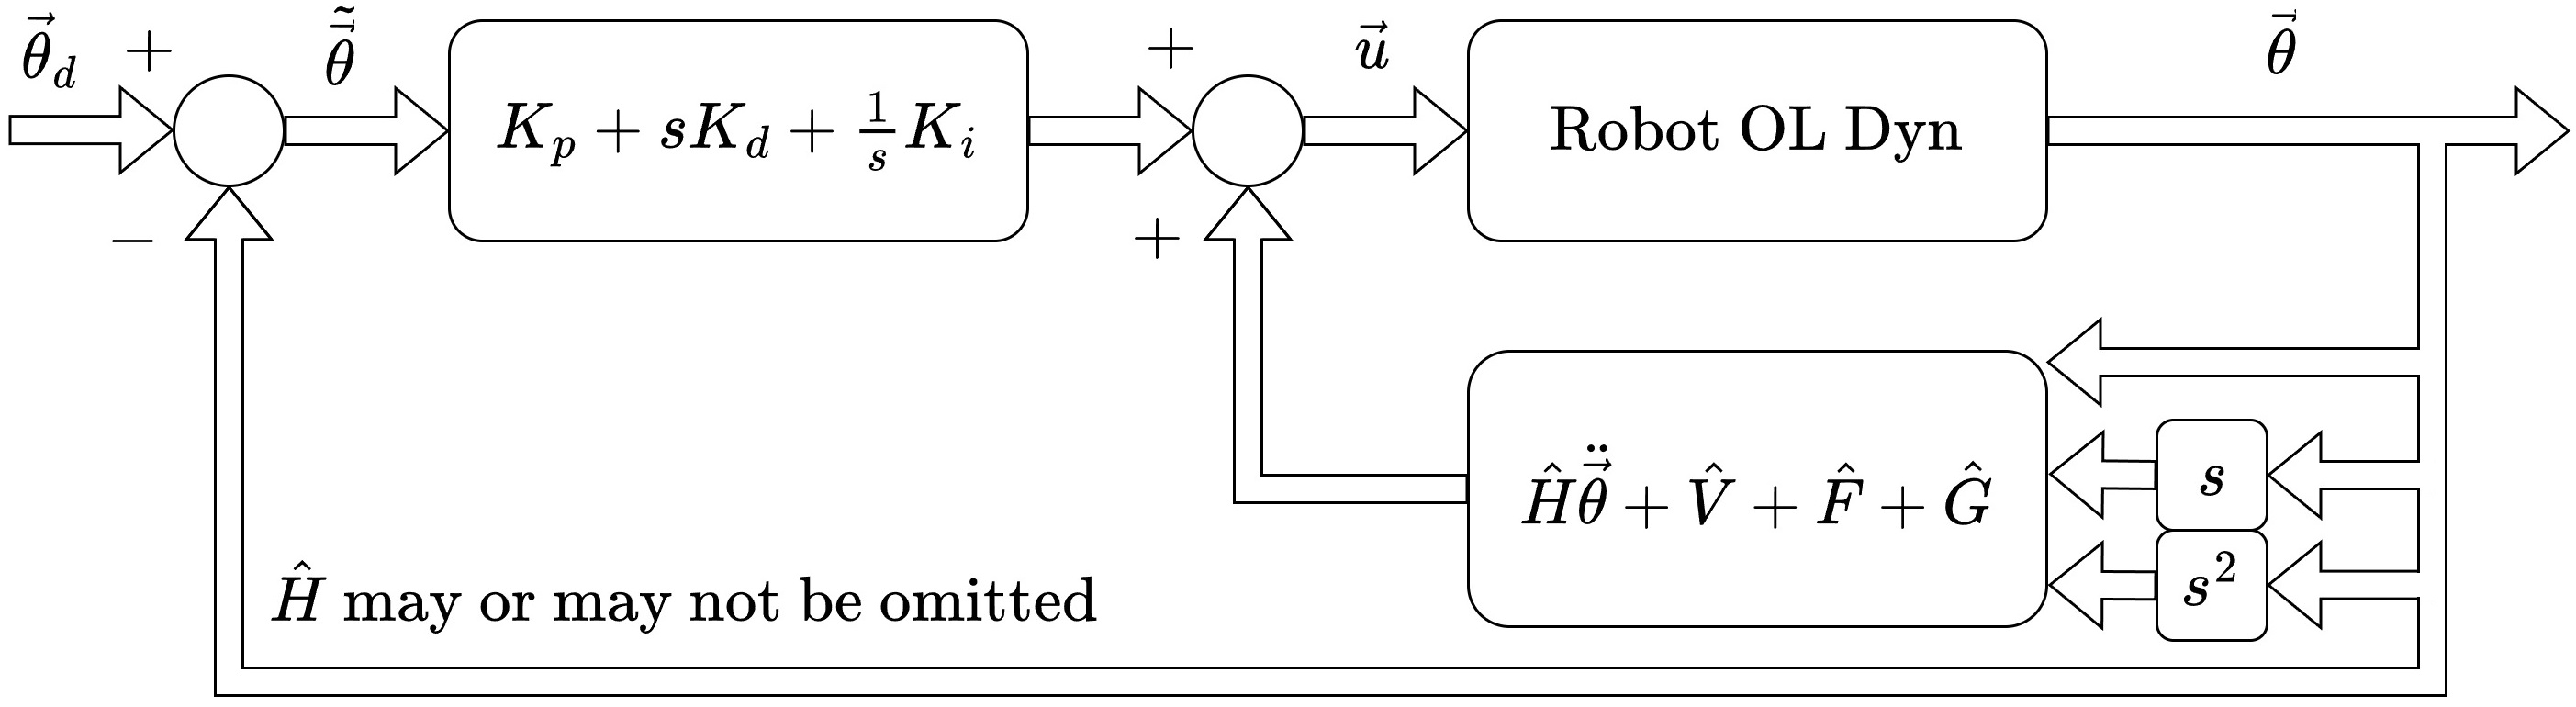
\includegraphics[width=0.49\textwidth]{figures/nl_feedback_comp.jpg}
\end{figure}
\end{comment}

\noindent\underline{Feedforward Computed Torque Control}\\
\begin{align*}
    \text{OL Dyn: }&
    \vec{\tau} = [\underbrace{I}_{\text{lin}} + \underbrace{H(\vec{\theta}) }_{\text{nonlin.}}]\ddot{\vec{\theta}} + \underbrace{V (\vec{\theta},\, \dot{\vec{\theta}})}_{\text{nonlin.}} + \underbrace{F(\dot{\vec{\theta}}) }_{\text{nonlin.}} + \underbrace{B\dot{\vec{\theta}} }_{\text{lin}} + \underbrace{G(\vec{\theta}) }_{\text{nonlin}}\\
    \text{Control law: }& \vec{\tau} = \left(K_p + sK_d + \frac{1}{s}K_i\right) \Tilde{\vec{\theta}}\\
    & \hspace{15pt} + \hat{H}(\vec{\theta}_d) \ddot{\vec{\theta}}_d + \hat{V}(\vec{\theta}_d,\, \dot{\vec{\theta}}_d) + \hat{F}(\dot{\vec{\theta}}_d) + \hat{G}(\vec{\theta}_d)
\end{align*}
\begin{figure}[h!]
    \centering
    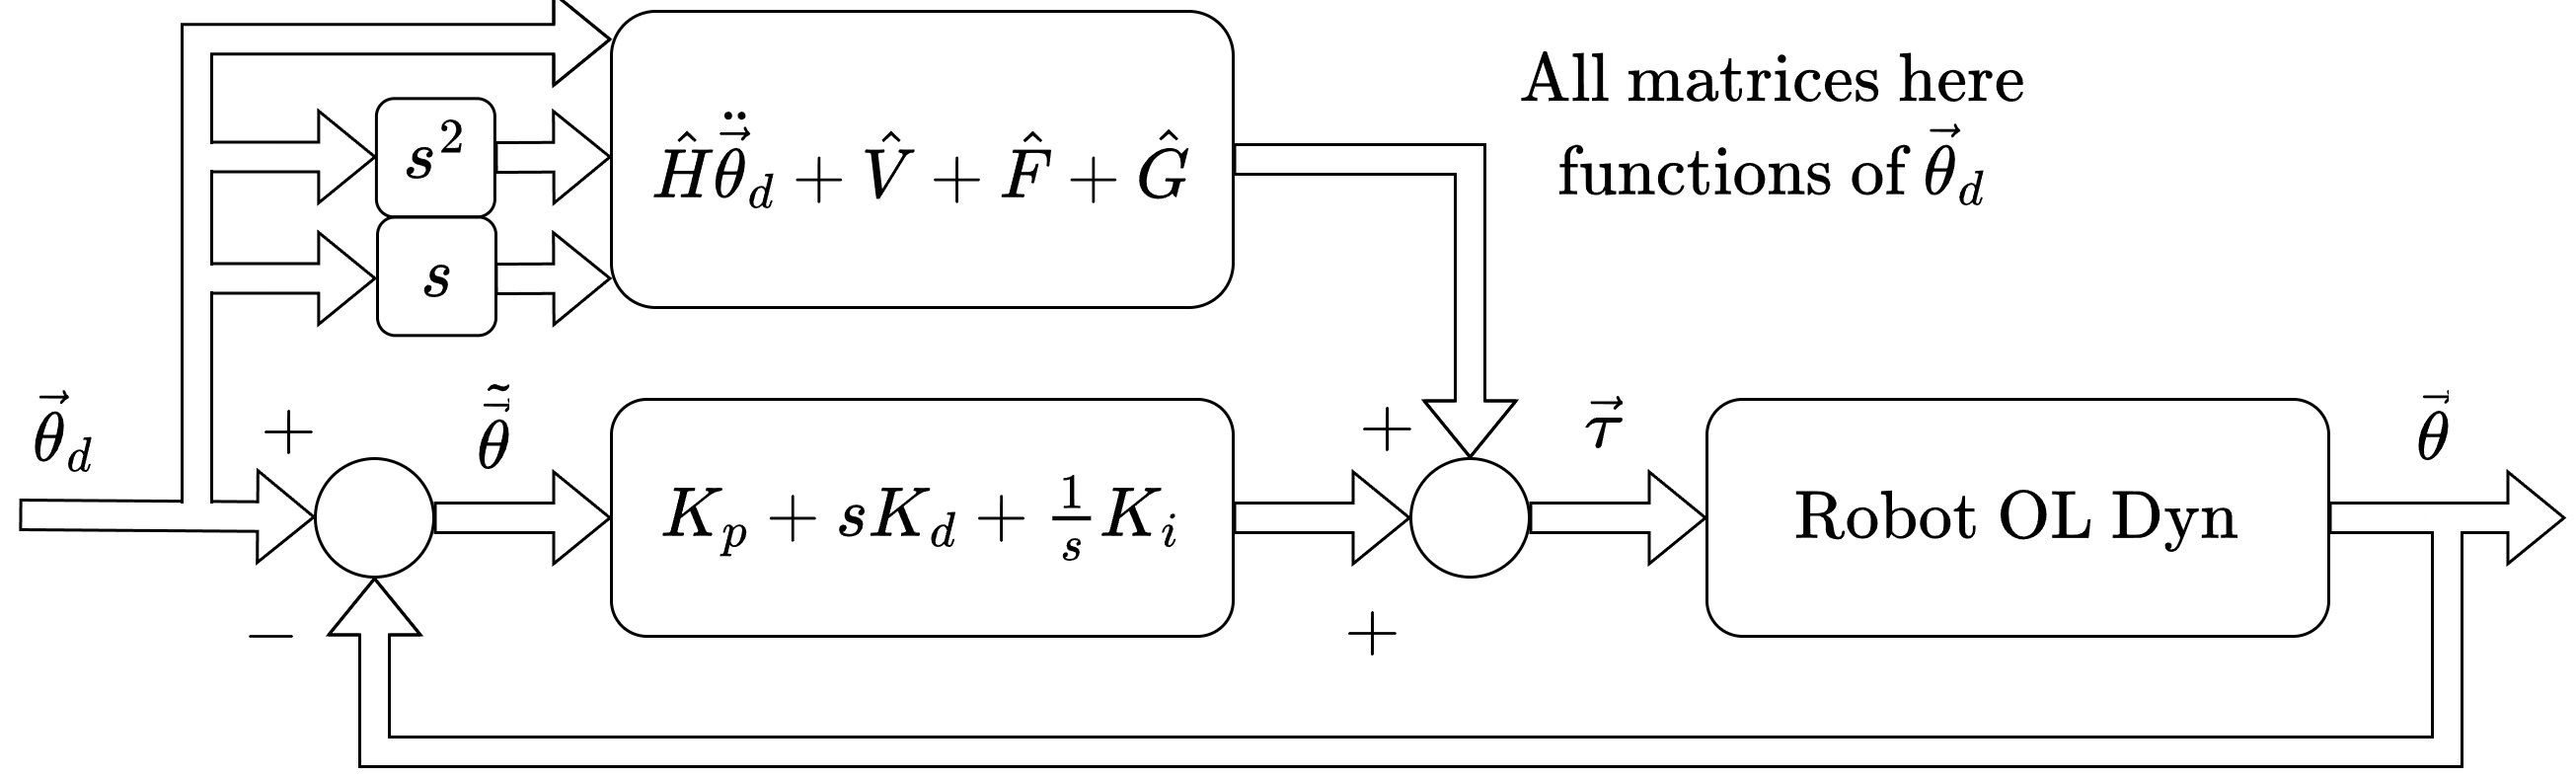
\includegraphics[width=0.49\textwidth]{figures/feedforward_ctc.jpg}
\end{figure}

\noindent\underline{Inverse Dynamic Control/Feedback Linearization}\\
Centralized control, accelerates \(\Tilde{\vec{\theta}}\) to zero. Removes dynamic coupling of error. \(\ddot{\vec{\theta}}_d\) is the desired acceleration, so \(\vec{\theta}_d =\vec{u}\). With perfect models, \(G_p(s) =1/s^2\) ,and perfect tracking.
\begin{align*}
    \text{OL Dyn: }&
    \vec{\tau} =  H(\vec{\theta})\ddot{\vec{\theta}} +\underbrace{V(\vec{\theta},\, \dot{\vec{\theta}}) + F(\dot{\vec{\theta}}) + G(\vec{\theta})}_{N(\vec{\theta},\, \dot{\theta})} \\
    \text{Control law: }& \vec{\tau} = \hat{H}(\vec{\theta}) \vec{u} + \hat{N}(\vec{\theta},\, \dot{\vec{\theta}})\\
    & \vec{u} = \left(K_p + sK_d + \frac{1}{s}K_i\right) \Tilde{\vec{\theta}}+ \ddot{\vec{\theta}}_d
\end{align*}
\begin{comment}
\begin{figure}[h!]
    \centering
    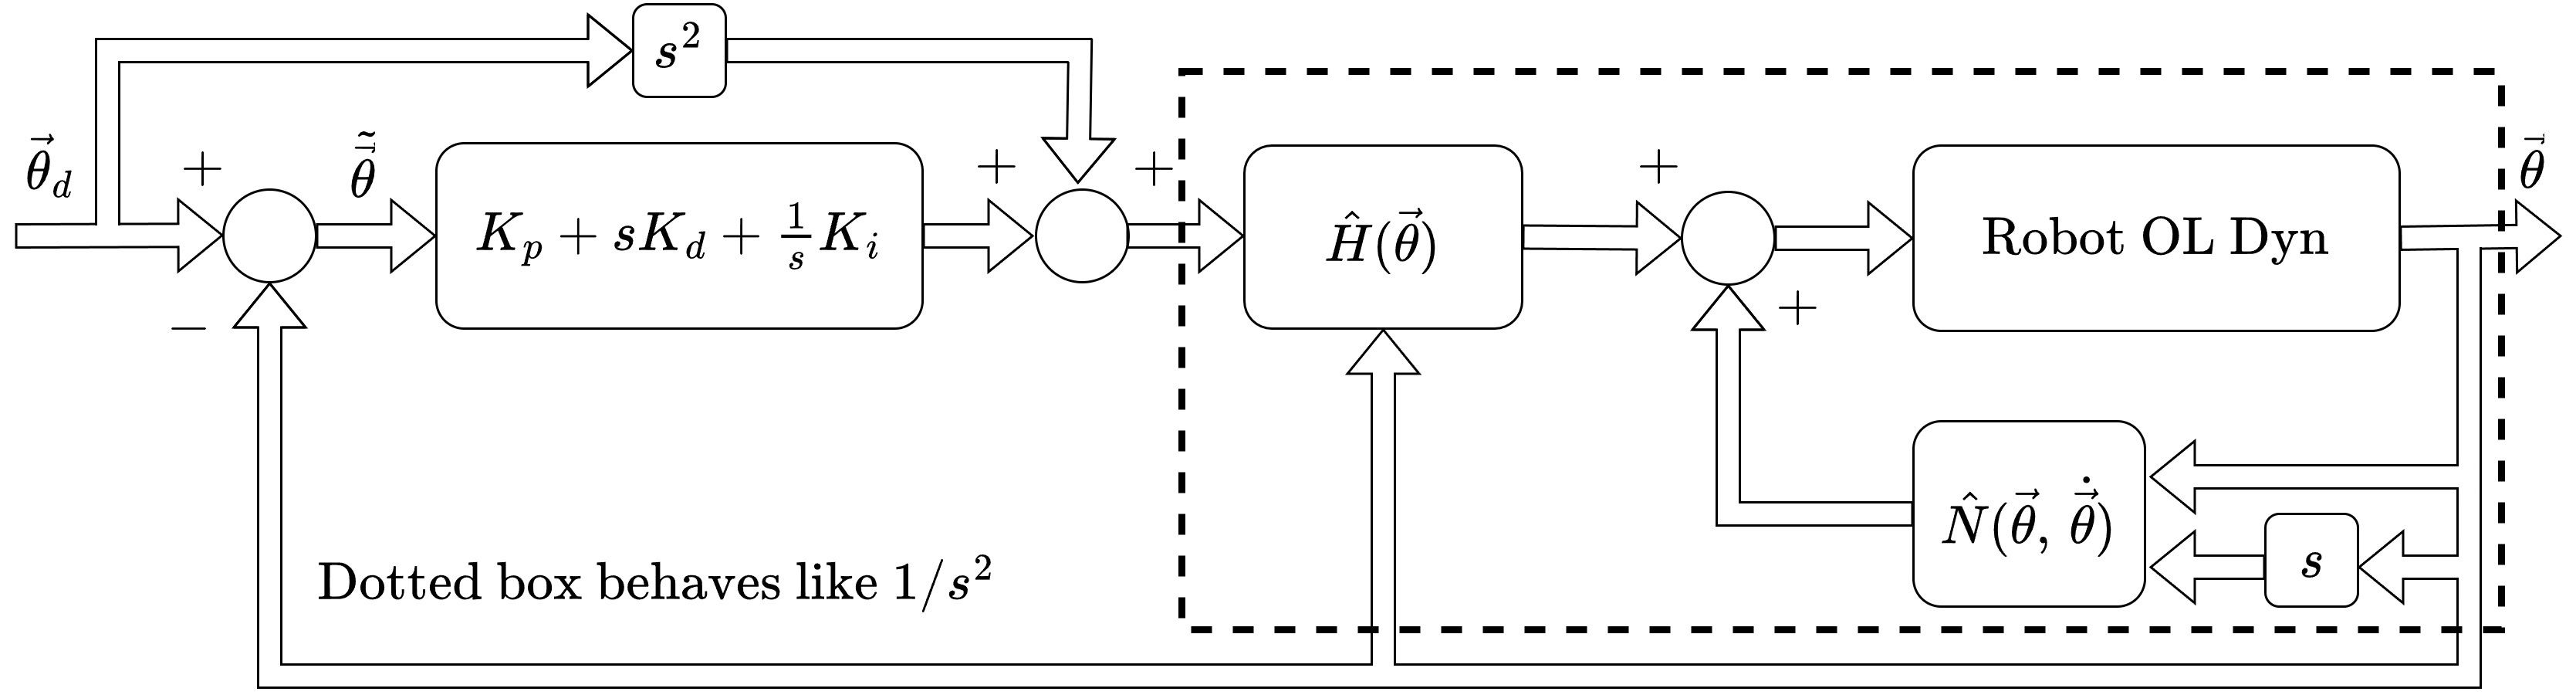
\includegraphics[width=0.49\textwidth]{figures/idc.jpg}
\end{figure}

\noindent\underline{Forward Dynamics Block}
\begin{figure}[h!]
    \centering
    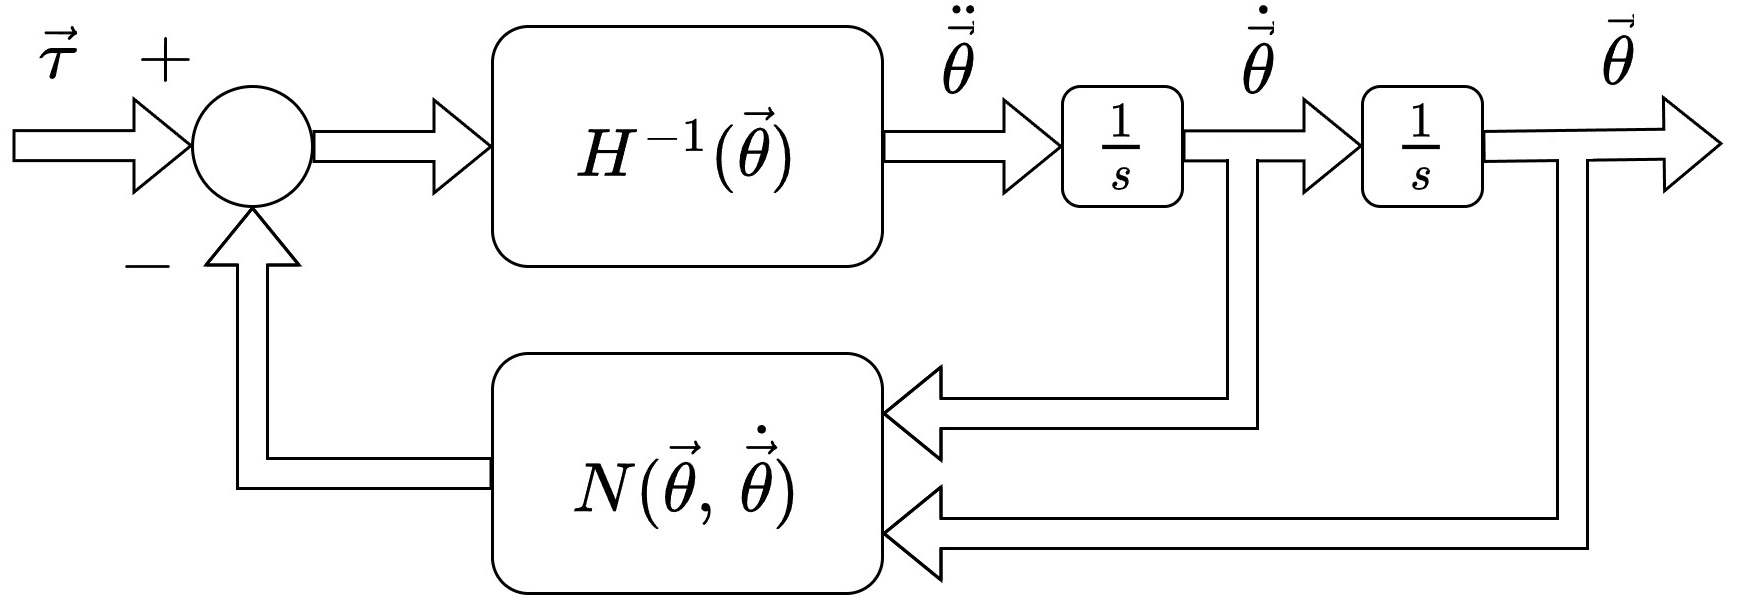
\includegraphics[width=0.40\textwidth]{figures/forward_dyn.jpg}
\end{figure}
\end{comment}

%%%%
\noindent\underline{Sliding Mode Control}\\
Pick \(\lambda_i \geq 5\times\) PD dyn. w/ \(\lambda_i\) the time const. of the sliding surface for joint \(i\). Set \(\varepsilon>\tilde{\theta}=\) width of allowable chatter
\begin{equation*}
    \Lambda = \text{diag}(\lambda_1,\, \dots,\,\lambda_n) \hspace{20pt}
    \rho \geq \|\text{model error}\|_{\max} = \text{ ``hardware sat.''}
\end{equation*}
\begin{align*}
    \text{OL Dyn: }& \tau = H(\theta) \ddot{\theta} + N(\theta,\, \dot{\theta})\\
    \text{Control law: }& \hat{\tau} = \hat{H}(\theta) u  + \hat{N}(\theta,\, \dot{\theta})
\end{align*}
\begin{figure}[h!]
    \centering
    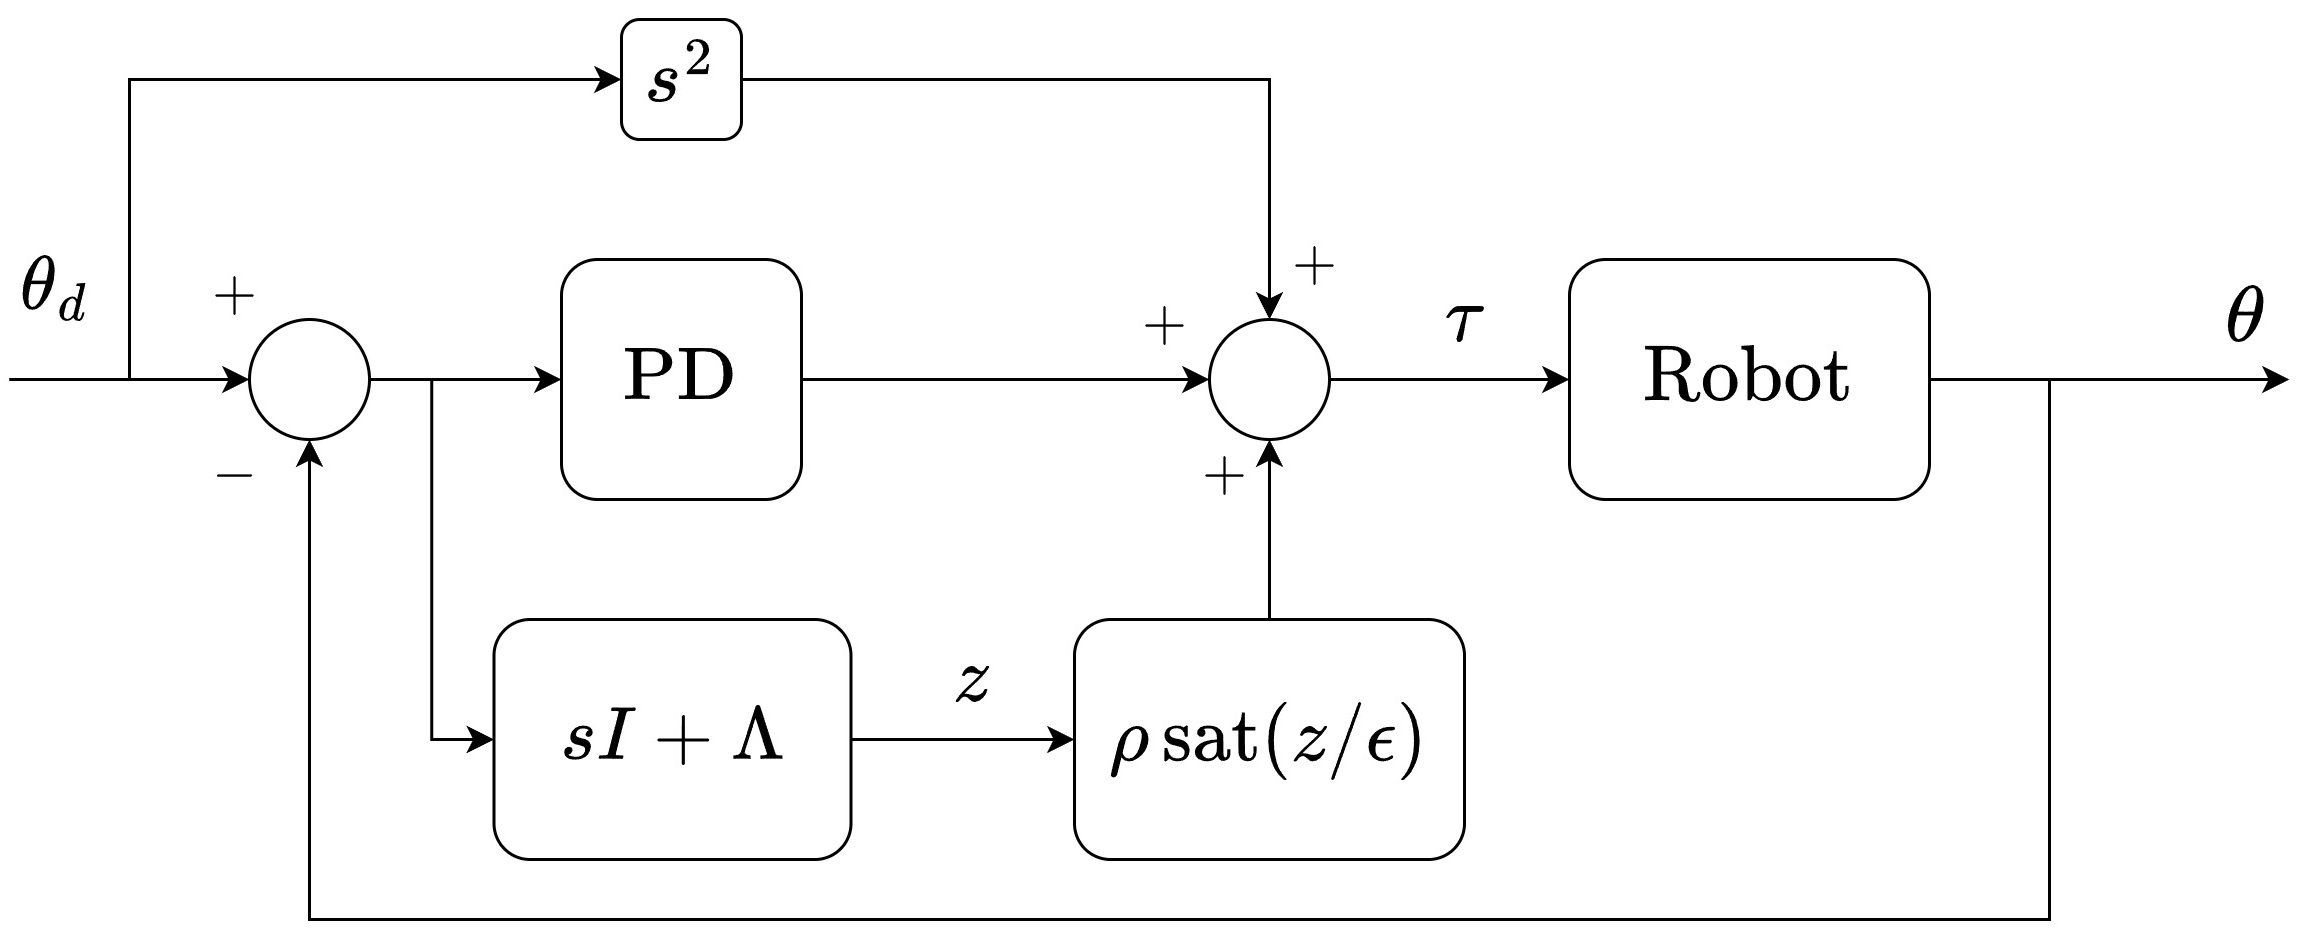
\includegraphics[width =0.45\textwidth]{figures/sliding_mode_control.jpg}
\end{figure}

%%
\newpage
\noindent\underline{Adaptive Control}\\
\(Y\) is chosen based upon the structured uncertainty terms \(\alpha\) such that \(\hat{\tau} = Y\hat{\alpha}\). \(Y\) will then be a function of whatever angles/signals necessary. To guarantee Lyapunov stability, ddots are replaced with ddot-reference, any centripetal/coriolis terms get one velocity replaced with dot-reference, and actual signals stay as measured.
\begin{equation*}
    \tau = \hat{\tau} + K_d (s\dot{\tilde{\theta}} + \Lambda \tilde{\theta}) \hspace{30pt} K_p = K_d \Lambda \hspace{30pt} \sigma = s\dot{\tilde{\theta}} + \Lambda \tilde{\theta} 
\end{equation*}
\begin{equation*}
    \hat{\tau}= Y\hat{\alpha} \hspace{30pt} \dot{\hat{\alpha}} = \Gamma^{-1} Y^T \sigma
\end{equation*}
\begin{align*}
    \text{OL Dyn: }& \tau = H(\theta) \ddot{\theta} + N(\theta,\, \dot{\theta})\\
    \text{Control law: }& \hat{\tau} = \hat{H}(\theta) u  + \hat{N}(\theta,\, \dot{\theta})
\end{align*}
\begin{figure}[h!]
    \centering
    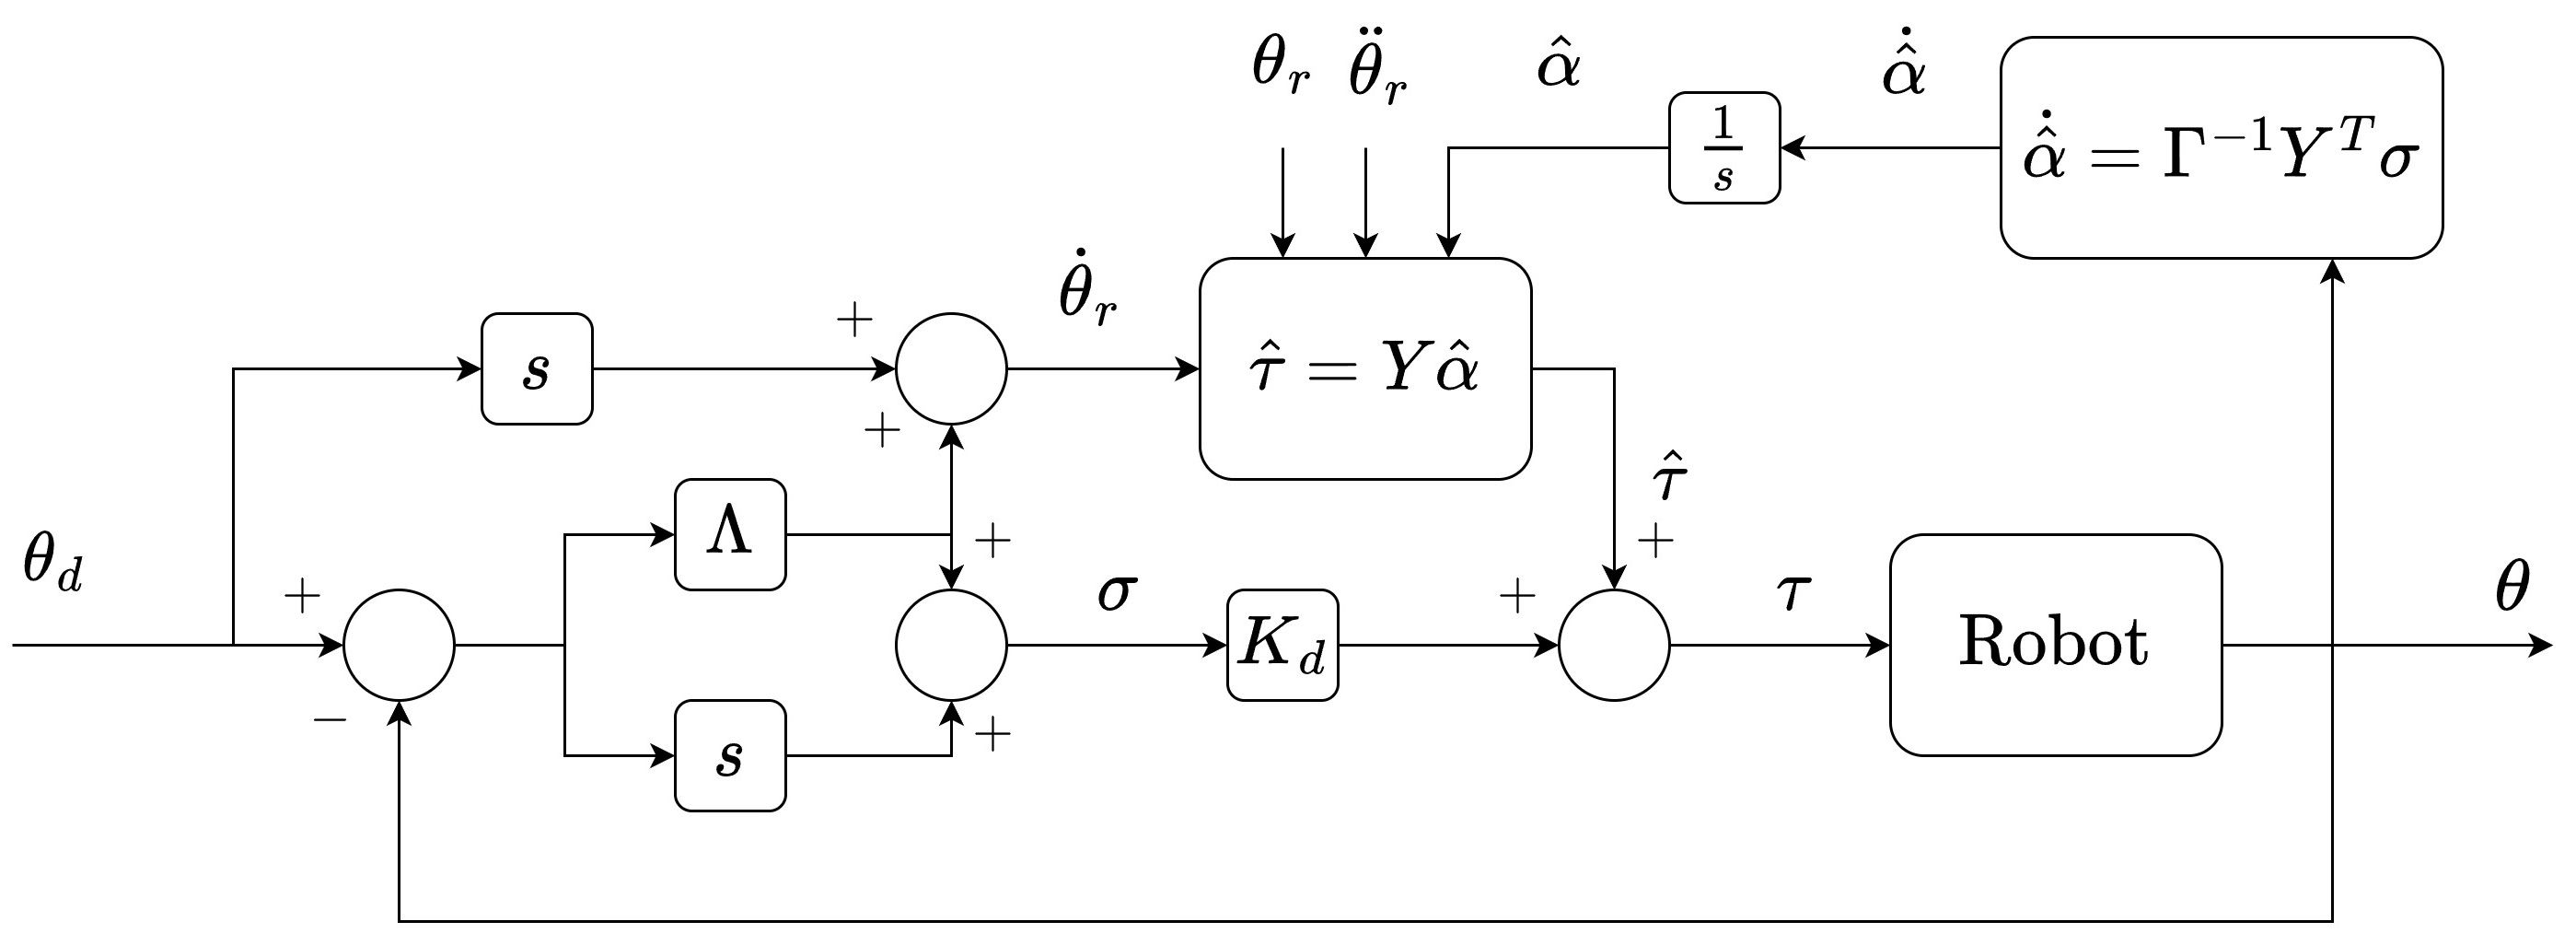
\includegraphics[width =0.45\textwidth]{figures/adaptive_control}
\end{figure}

%%%
\noindent\underline{Jacobian Inverse/Transpose Control}
\begin{equation*}
    \text{Doesn't require IK.} \hspace{5pt} \dot{x} = J(\theta)\dot{\theta} \hspace{5pt} \Longrightarrow \hspace{5pt} \Delta x \approx J(\theta) \Delta \theta  \hspace{5pt} \Longrightarrow \hspace{5pt} \tilde{\theta} \approx J^{-1}(\theta) \tilde{x} 
\end{equation*}
\begin{figure}[h!]
    \centering
    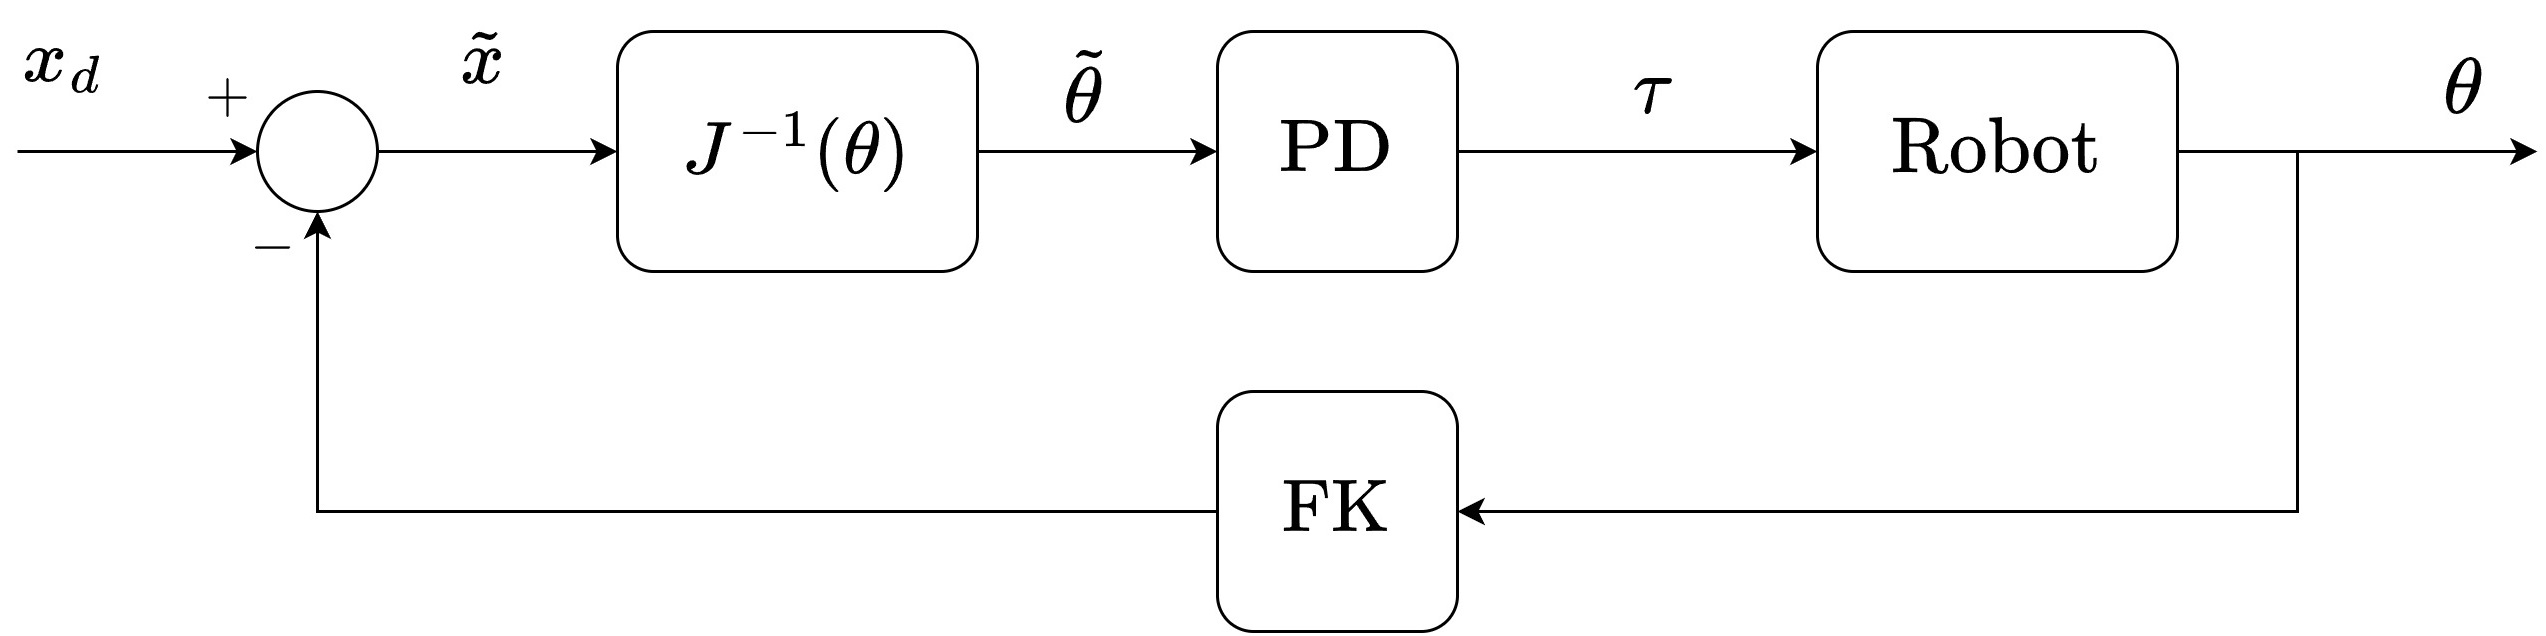
\includegraphics[width =0.45\textwidth]{figures/Jacobian_inverse.jpg}
\end{figure}
\begin{figure}[h!]
    \centering
    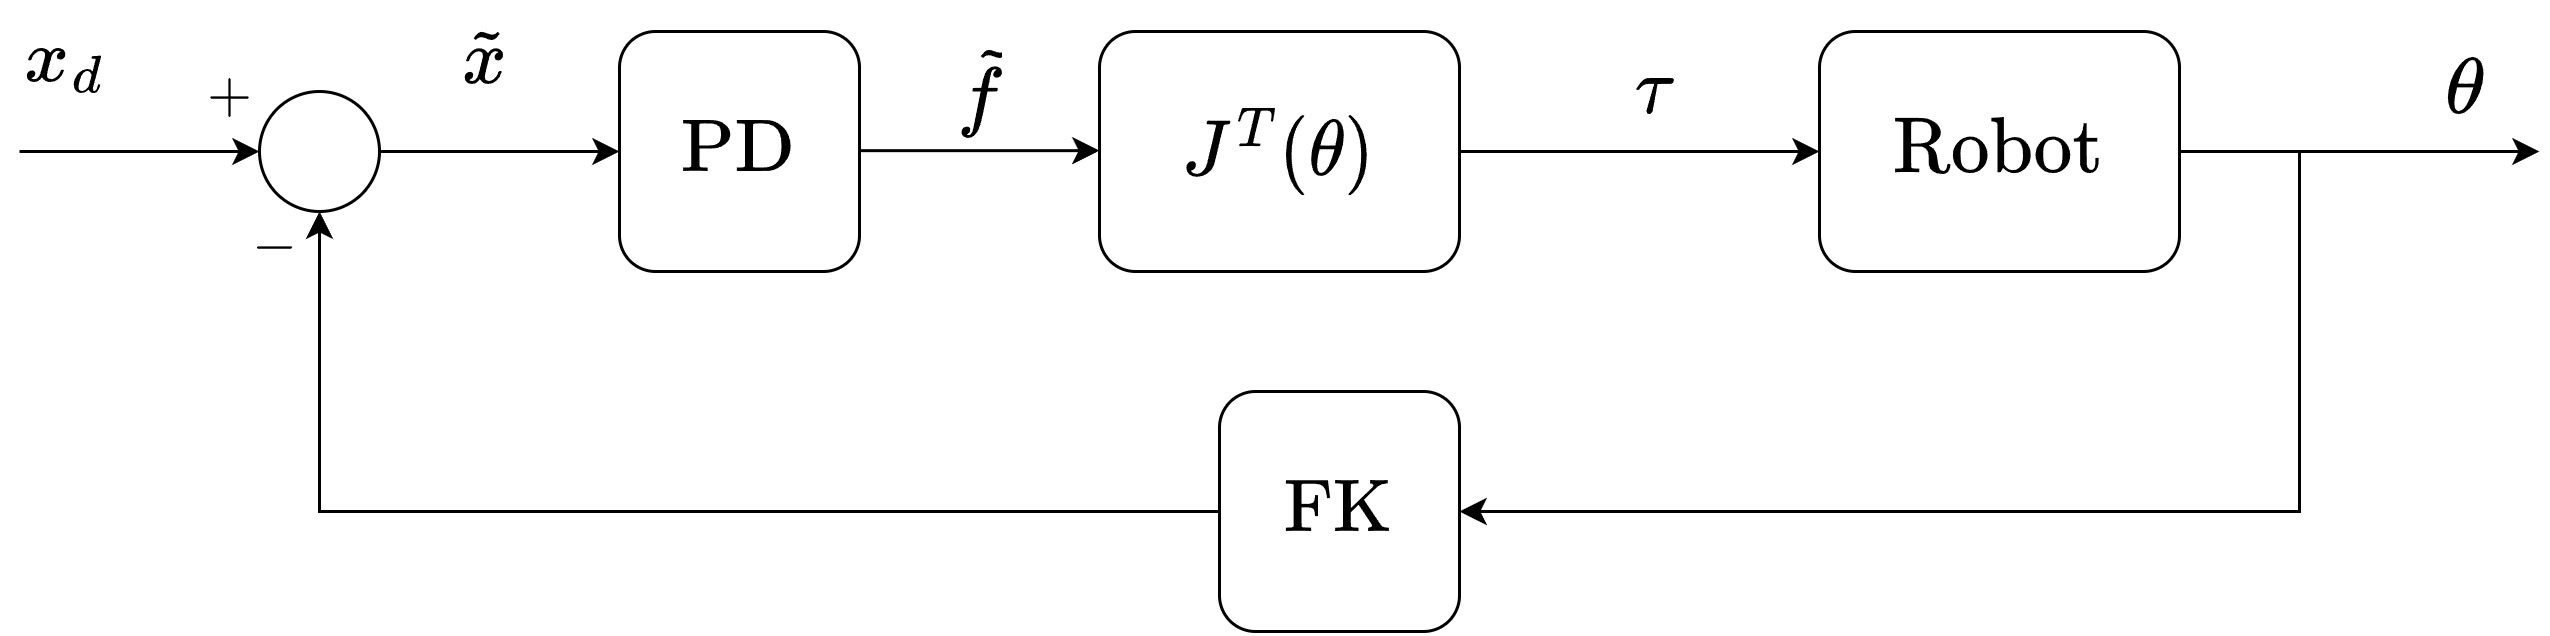
\includegraphics[width =0.45\textwidth]{figures/Jacobian_transpose.jpg}
\end{figure}

%%%%
\newpage
\noindent\underline{IDC in Op-Space}
\begin{equation*}
    \text{Sys. behaves like } 1/s^2  \hspace{20pt} \prescript{x}{}{\hat{H}}(\theta) = J^{-T}(\theta) \hat{H}(\theta) J^{-1}(\theta)
\end{equation*}
\begin{figure}[h!]
    \centering
    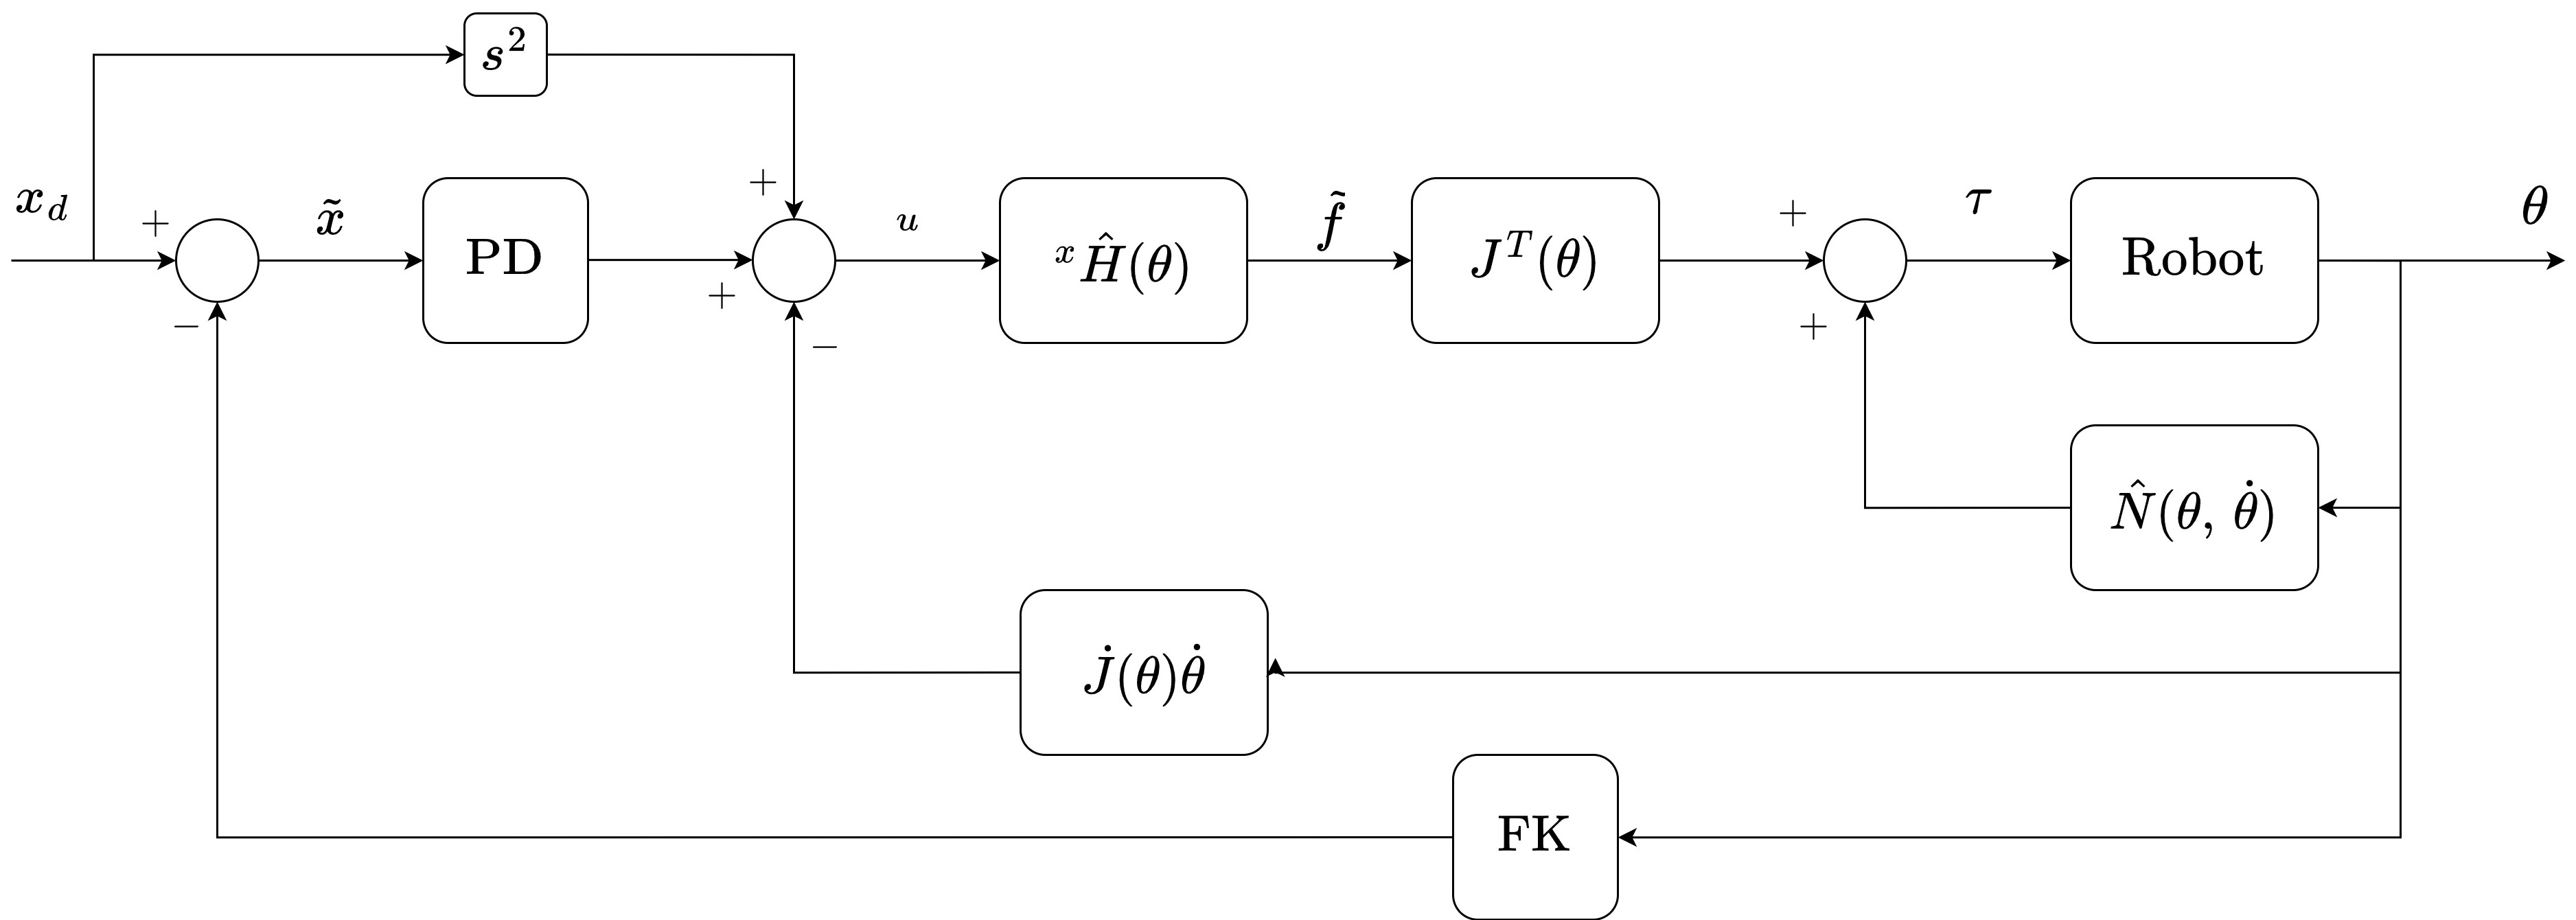
\includegraphics[width =0.45\textwidth]{figures/idc_op_space.jpg}
\end{figure}

%%%%
% \newpage
\noindent\underline{Feedforward Force Control (direct)}
\begin{figure}[h!]
    \centering
    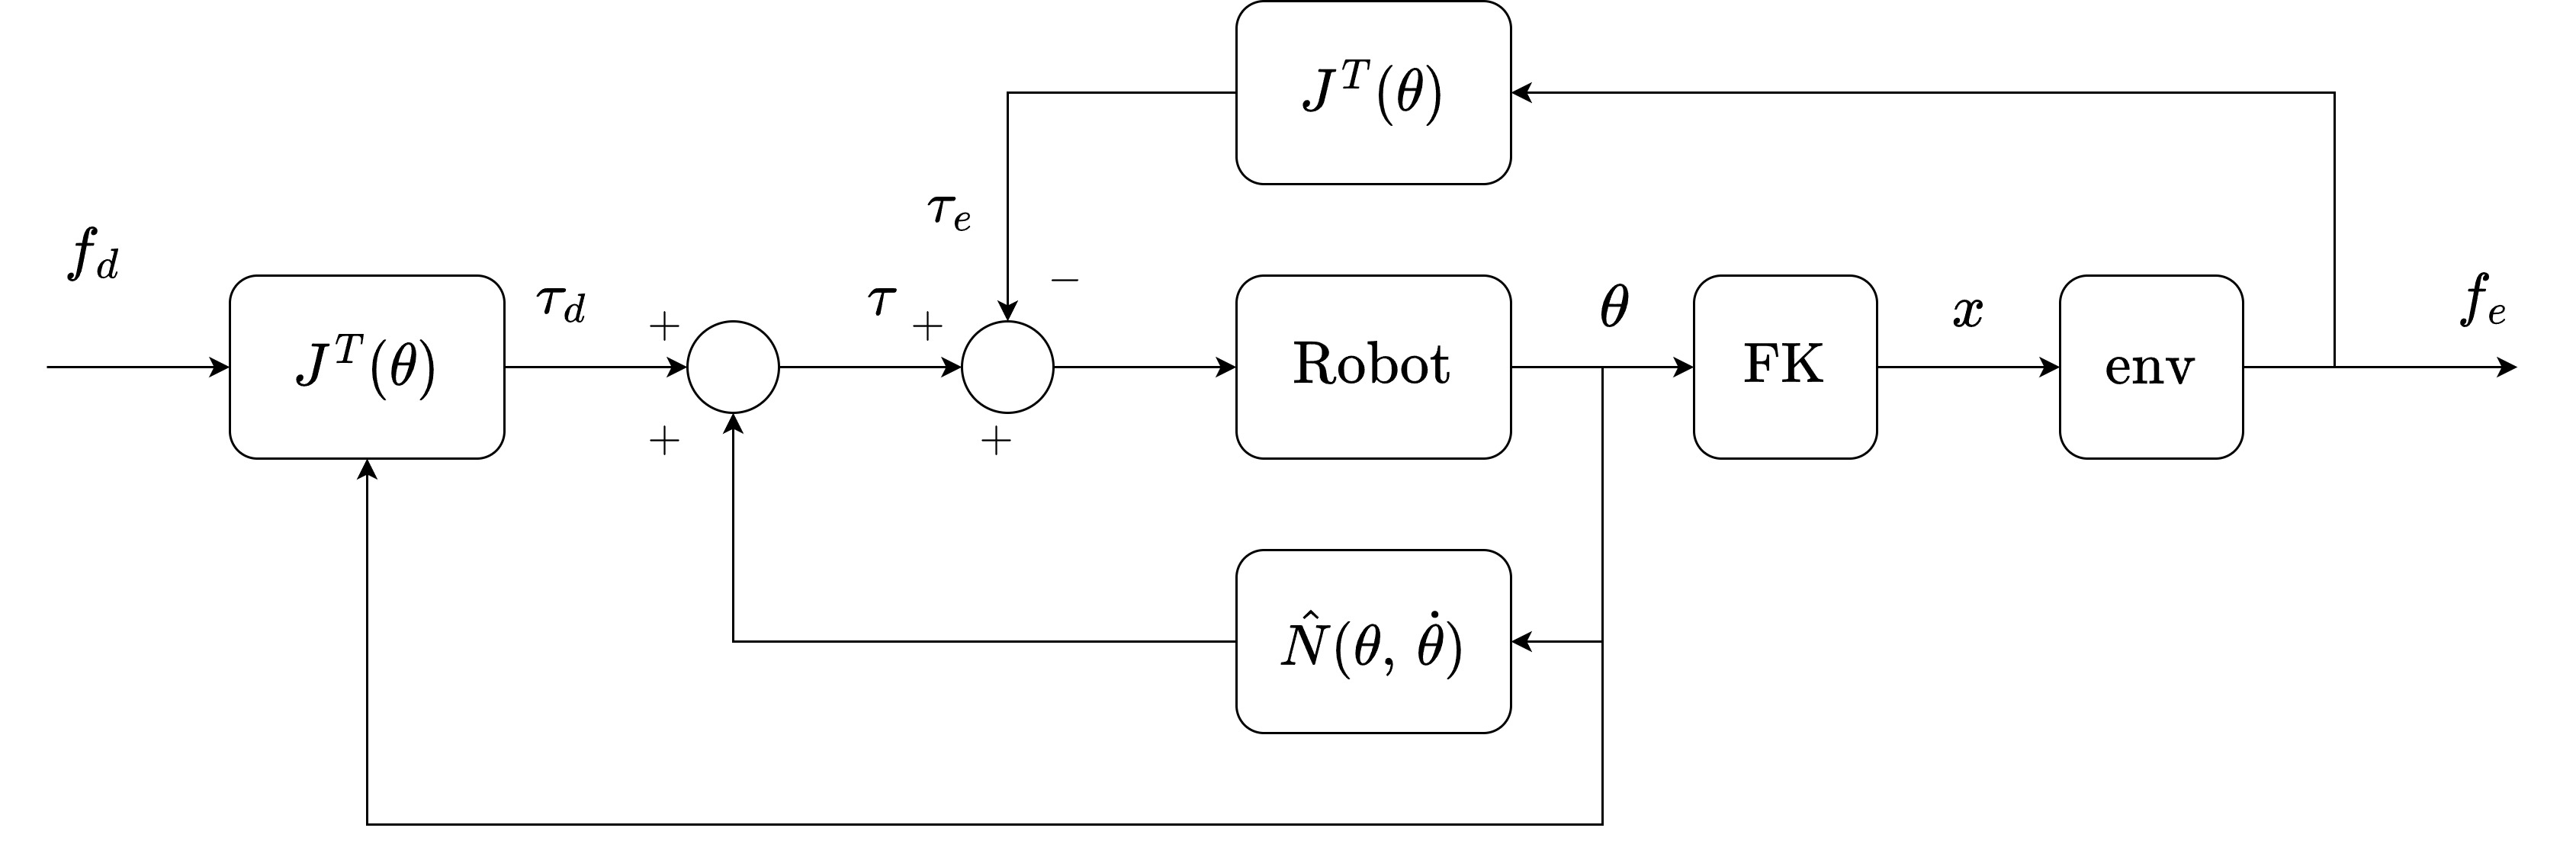
\includegraphics[width =0.45\textwidth]{figures/ff_force_control.jpg}
\end{figure}


%%%%
\noindent\underline{Stiffness/Damping Control (indirect)}\\
Programmable stiffness/damping. Feels like sping/damper at EE
\begin{figure}[h!]
    \centering
    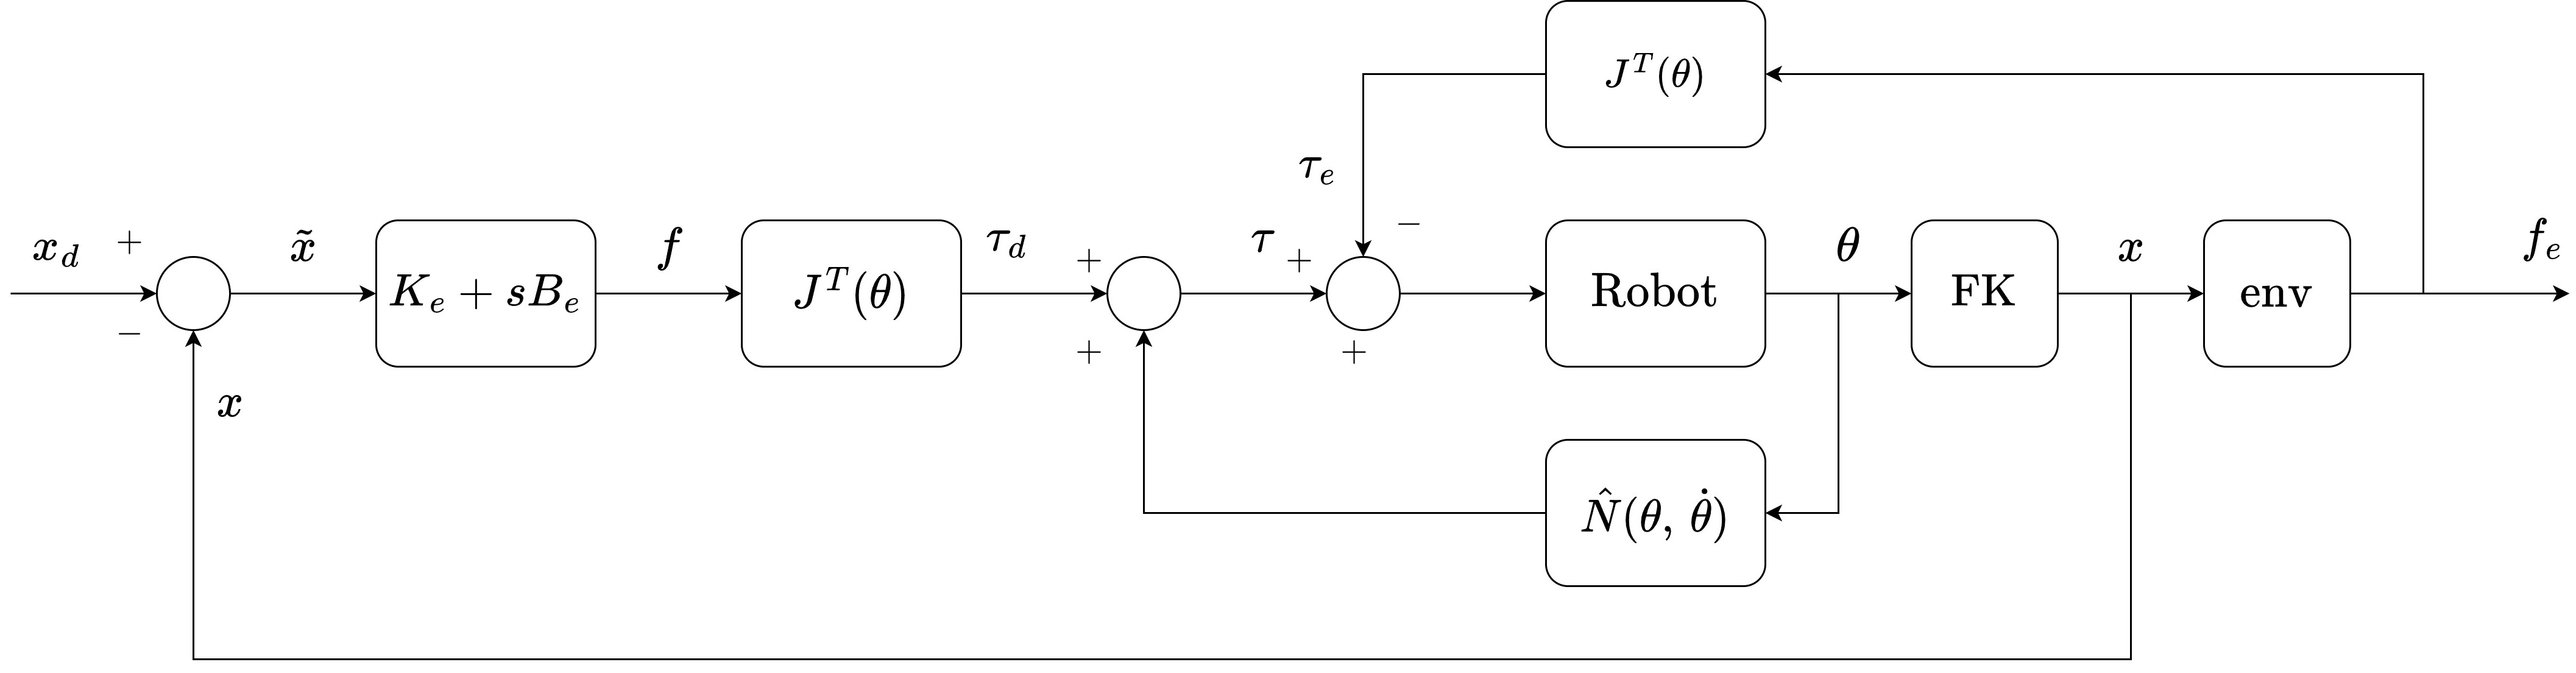
\includegraphics[width =0.45\textwidth]{figures/stiffness_control.jpg}
\end{figure}

%%%%
\noindent\underline{Impedance Control (indirect)}\\
Softening PD gains results in poor tracking and dist. rej. If robot is not back-drivable, works poorly, as hard to displace.
\begin{figure}[h!]
    \centering
    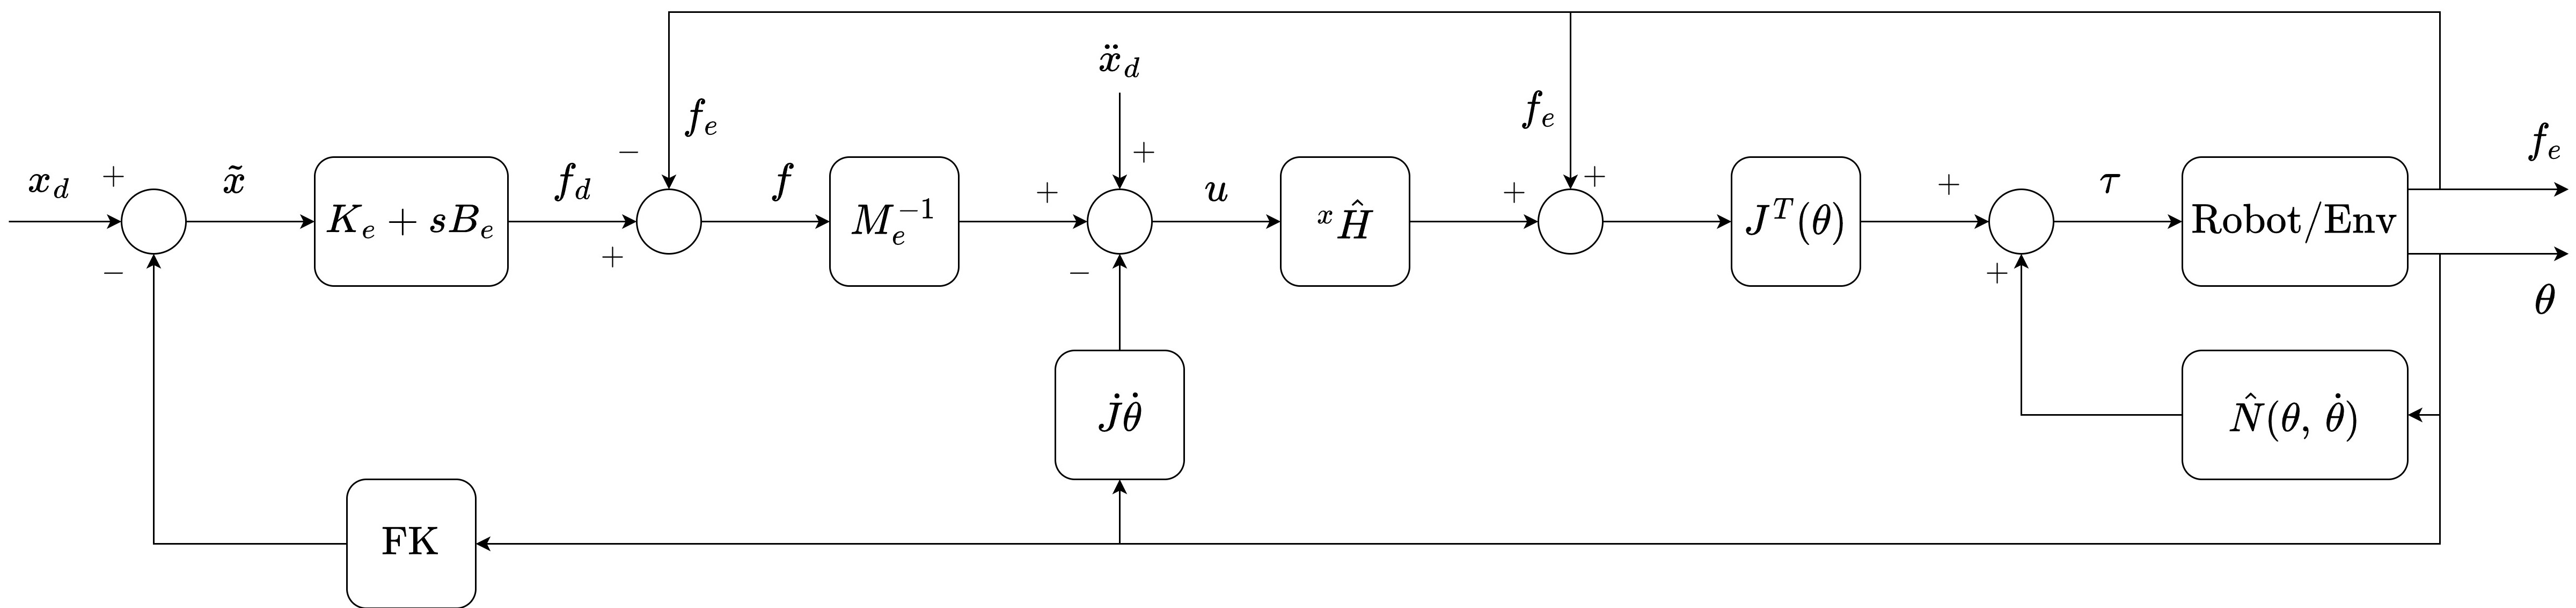
\includegraphics[width =0.45\textwidth]{figures/impedance_control.jpg}
\end{figure}

%%%%
\noindent\underline{Admittance Control (direct)}\\
PD gains stay high. \(C\) altered to affect behavior. NOT Lyapunov stable. Design \(A(s)\) to have desired 2\(^{\text{nd}}\) order characteristics.
\begin{figure}[h!]
    \centering
    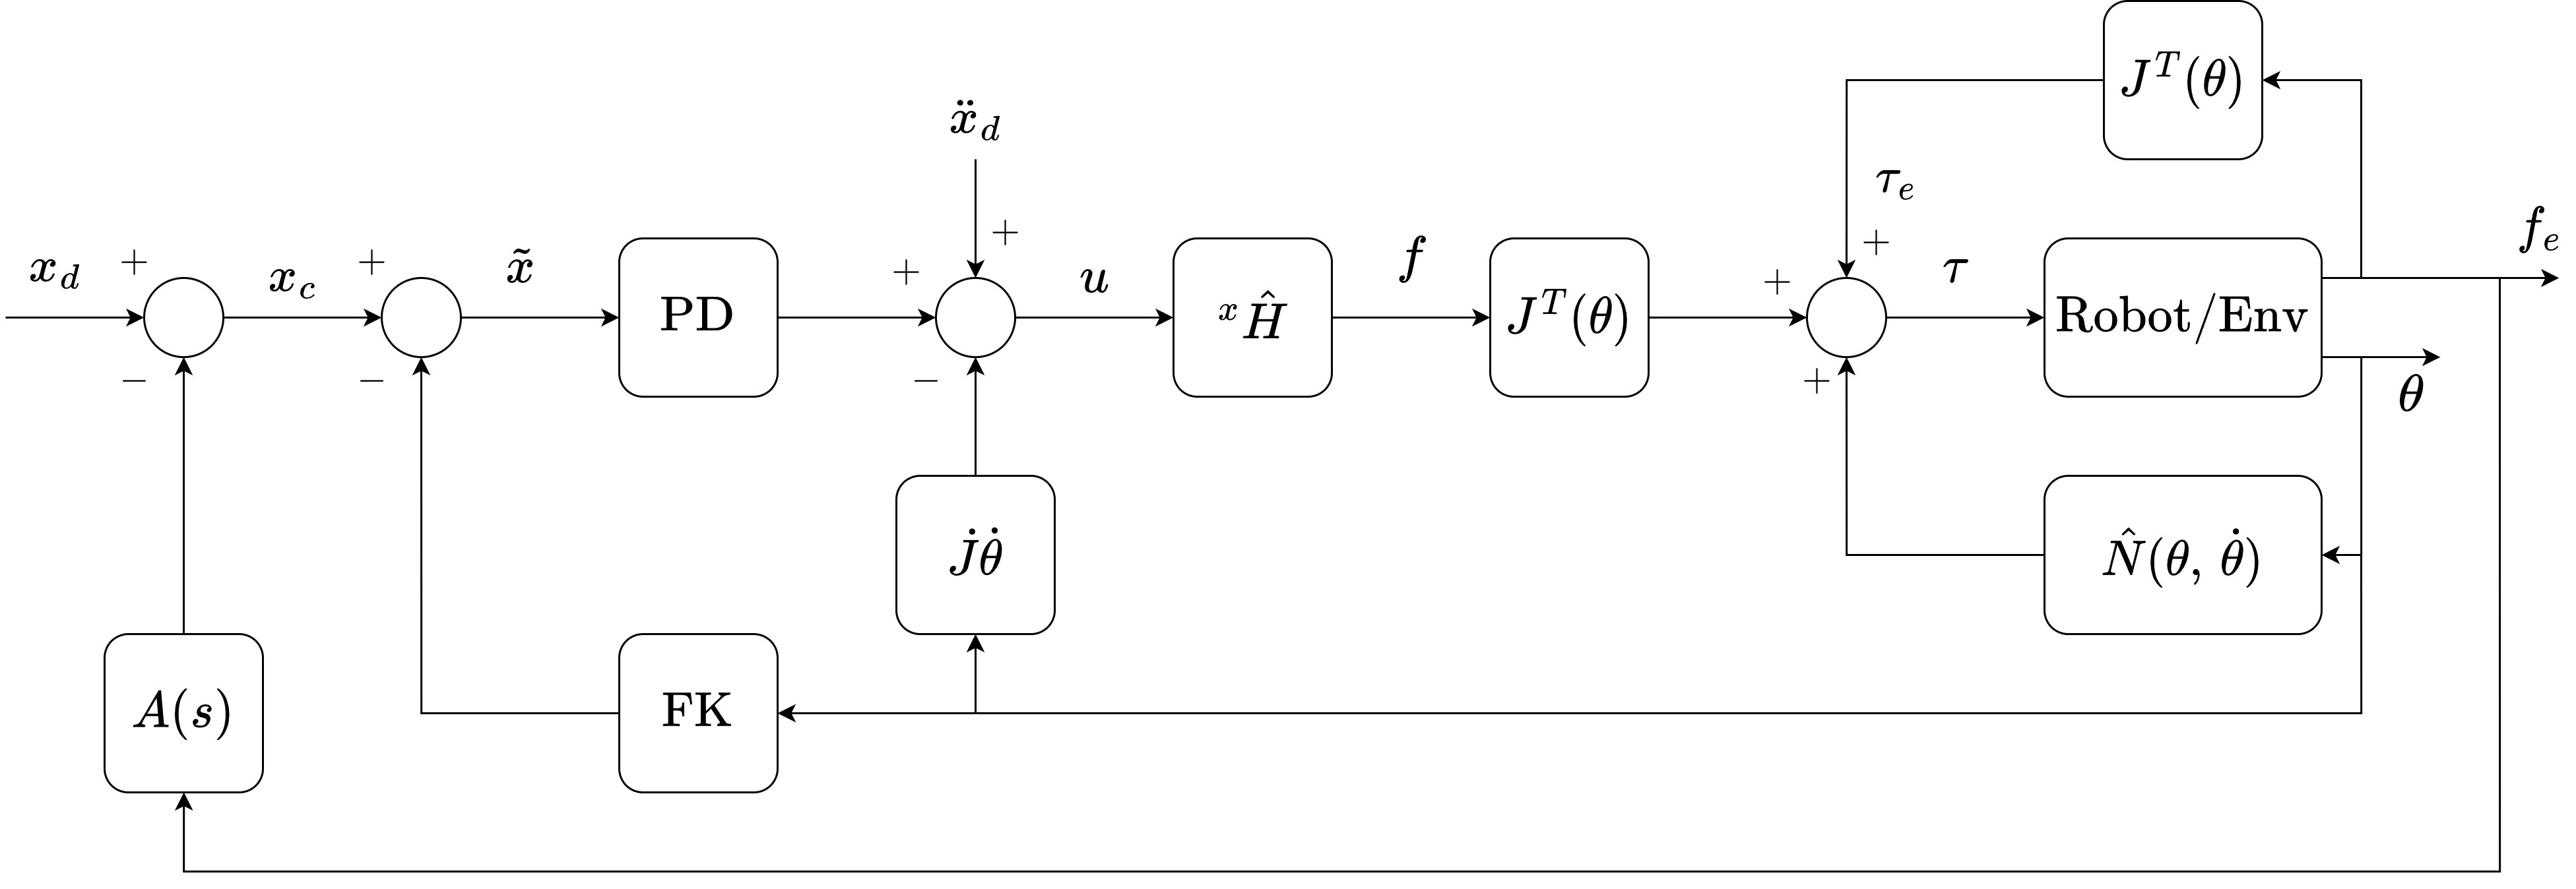
\includegraphics[width =0.45\textwidth]{figures/admittance_control.jpg}
\end{figure}

%%%%
\noindent\underline{Direct Force Control (direct)}\\
NOT Lyapunov stable, as \(k_pk_w\) appears in char. eq./loop gain
\begin{figure}[h!]
    \centering
    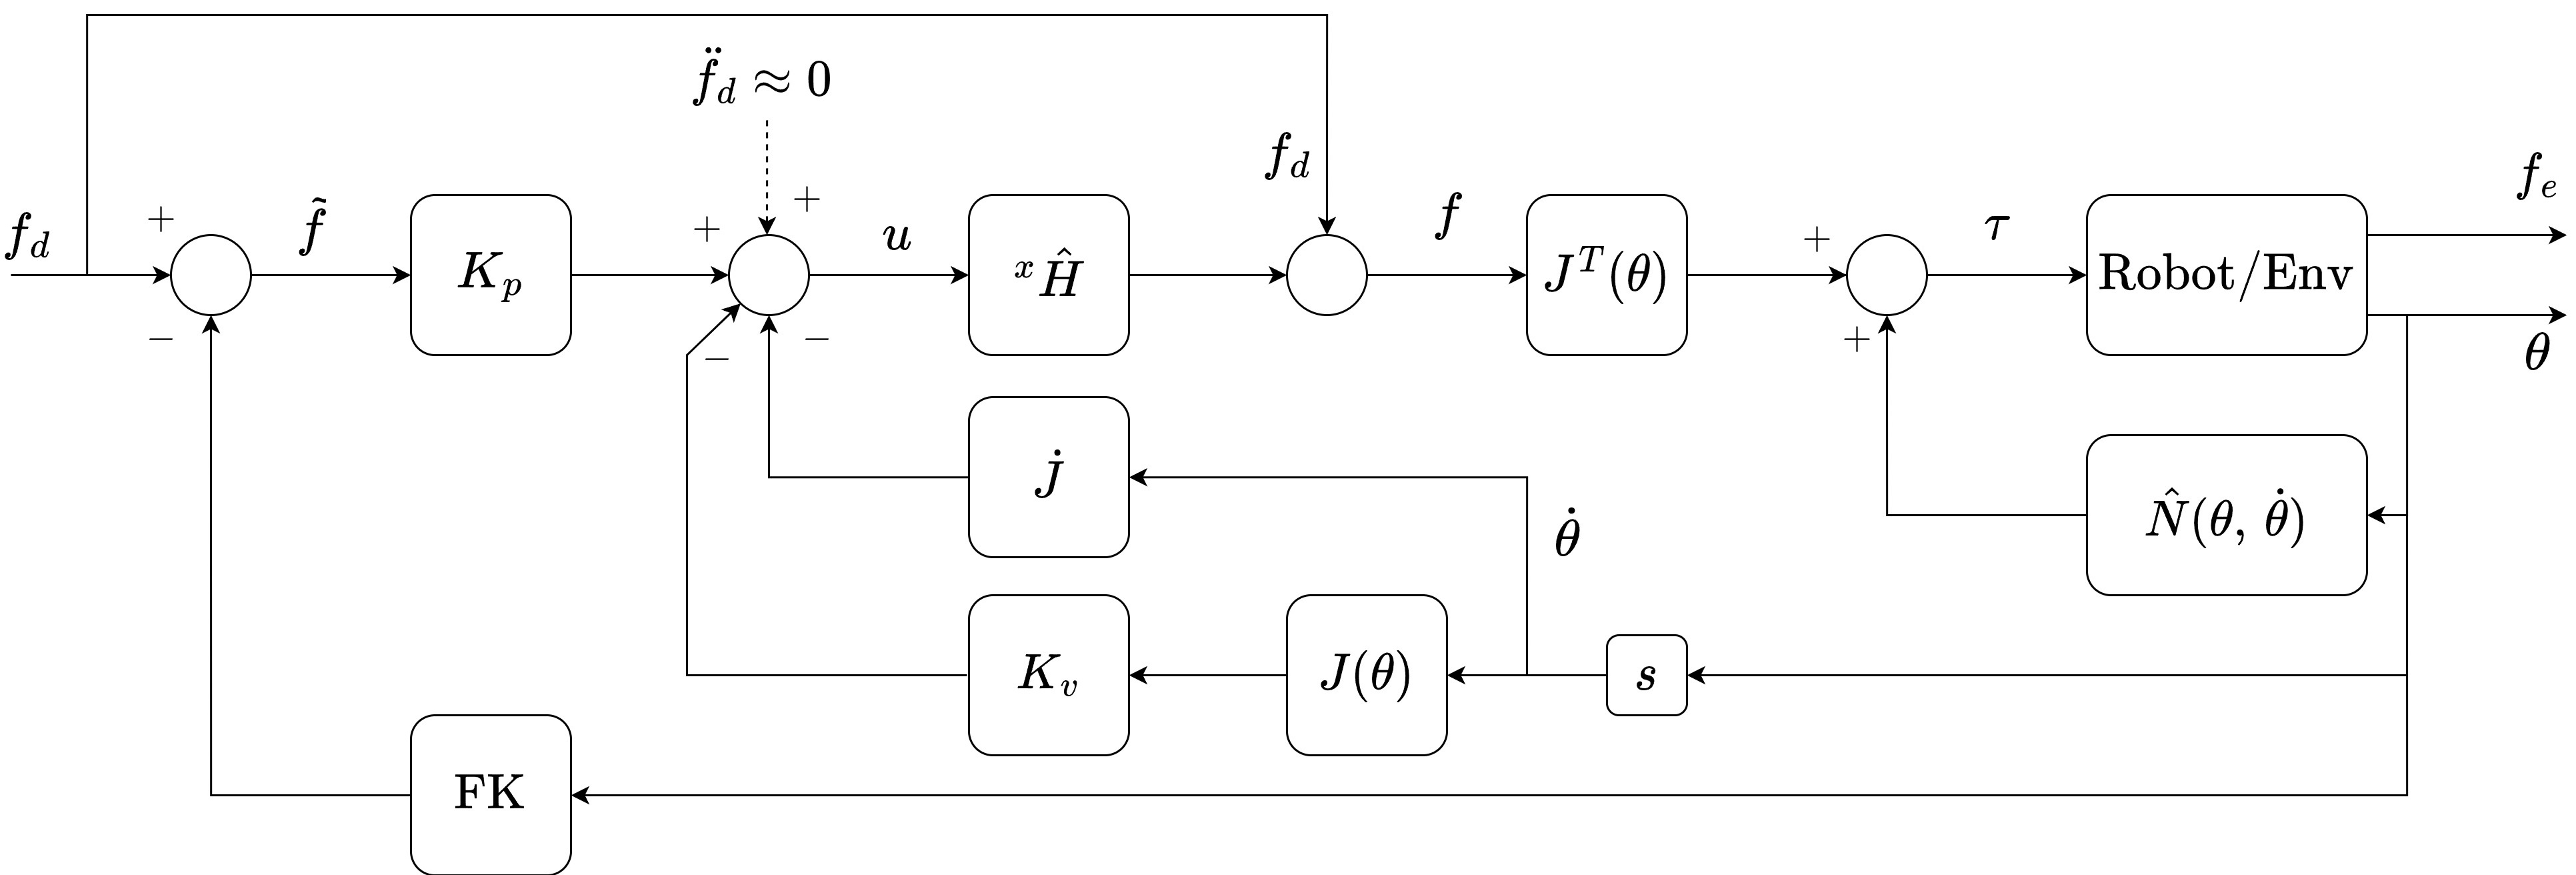
\includegraphics[width =0.45\textwidth]{figures/direct_force_control.jpg}
\end{figure}

%%%%
\newpage
\noindent\underline{Hybrid/Multi-Arm Control (direct)}
\begin{figure}[h!]
    \centering
    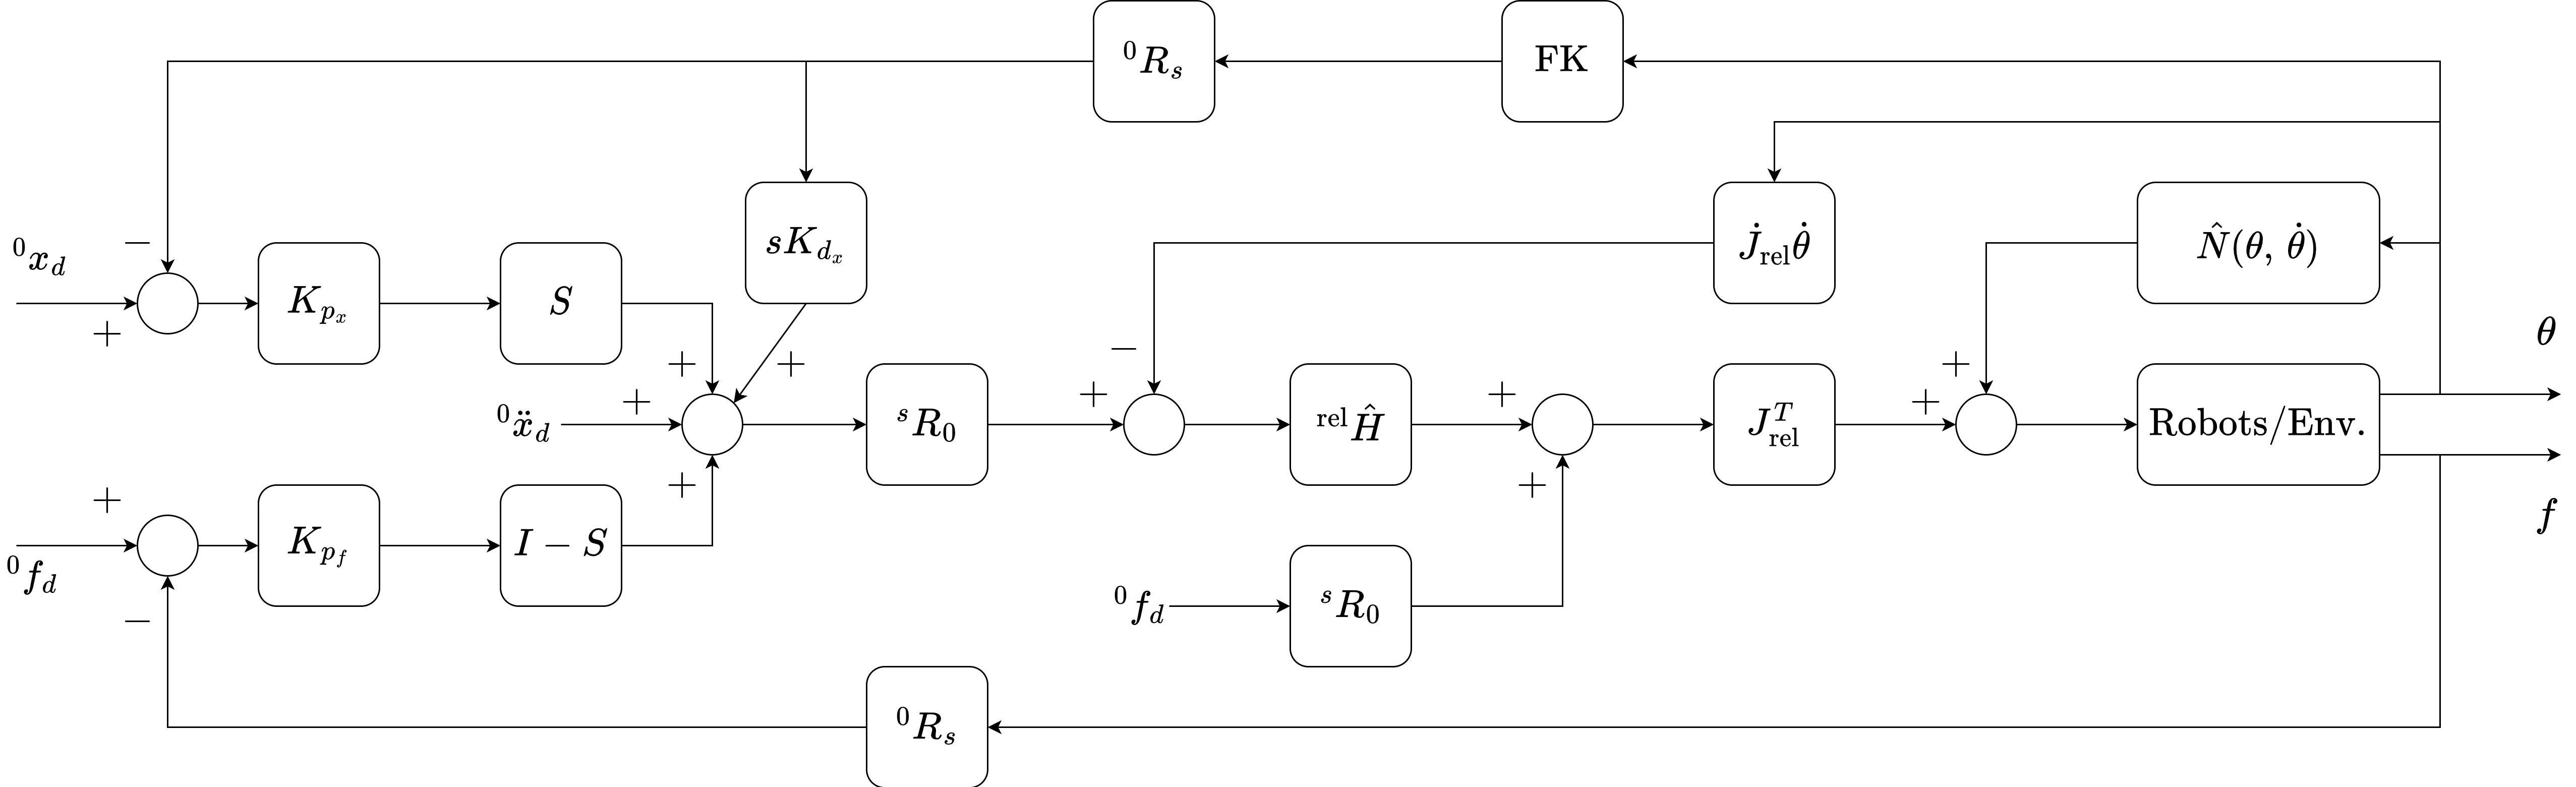
\includegraphics[width =0.45\textwidth]{figures/hybrid_control.jpg}
\end{figure}

%%%%
\noindent\underline{Bilateral (Servo Joint-Space [L]. Servo/Direct Force Op-Space [R])}

\begin{figure}[h!]
    \centering
    \begin{subfigure}{0.24\textwidth}
        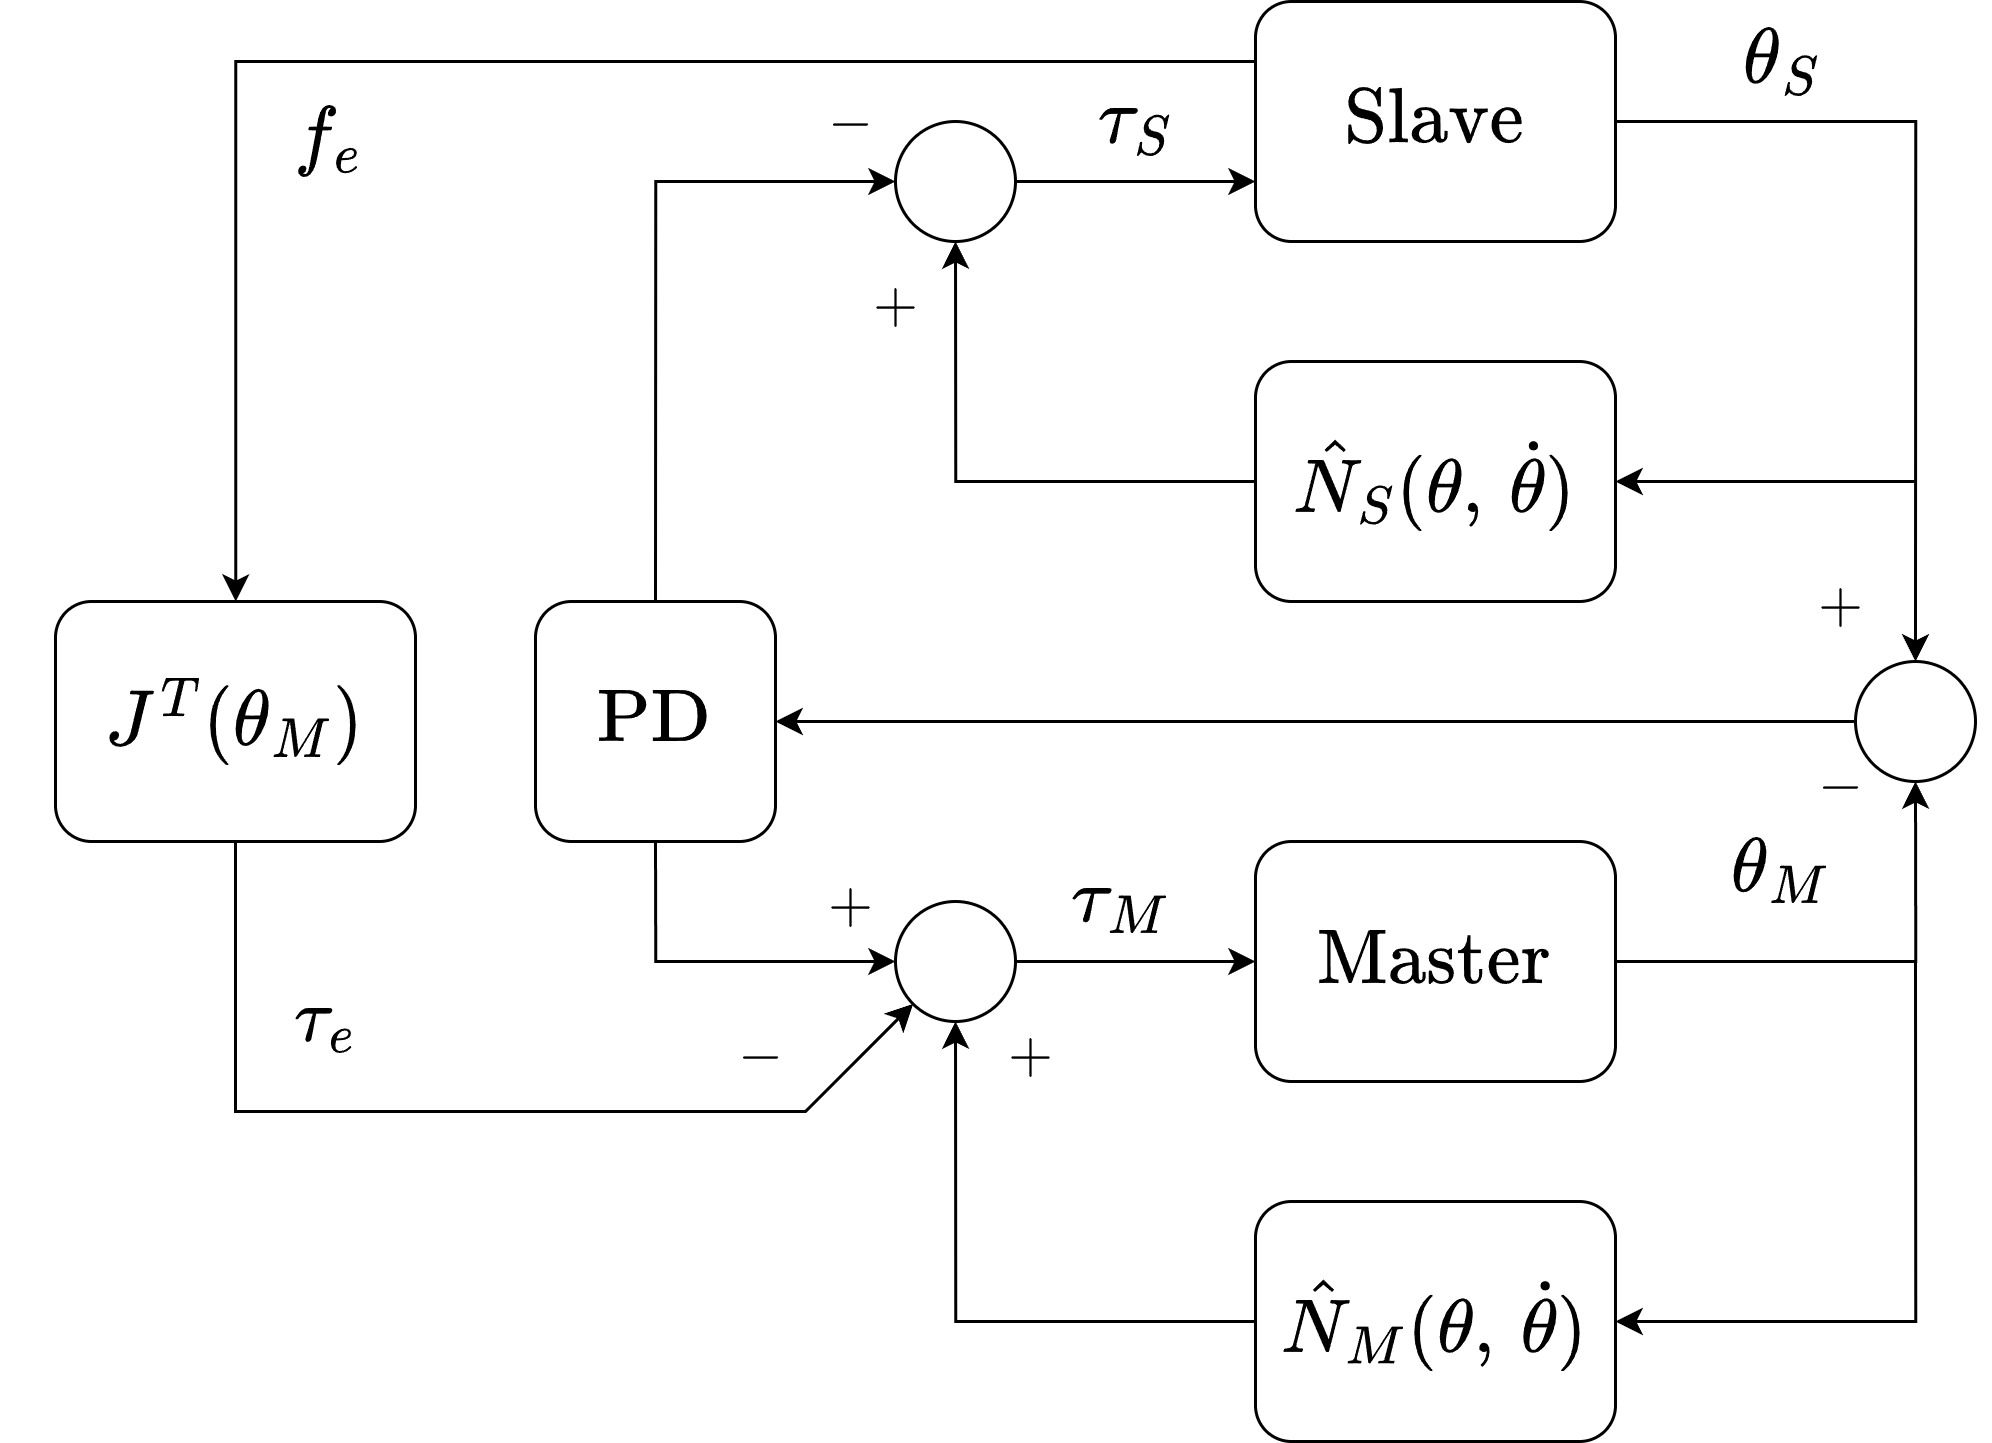
\includegraphics[width=\textwidth]{figures/bilateral_servo_direct_force_joint.jpg}
    \end{subfigure}
    \hfill
    \begin{subfigure}{0.24\textwidth}
        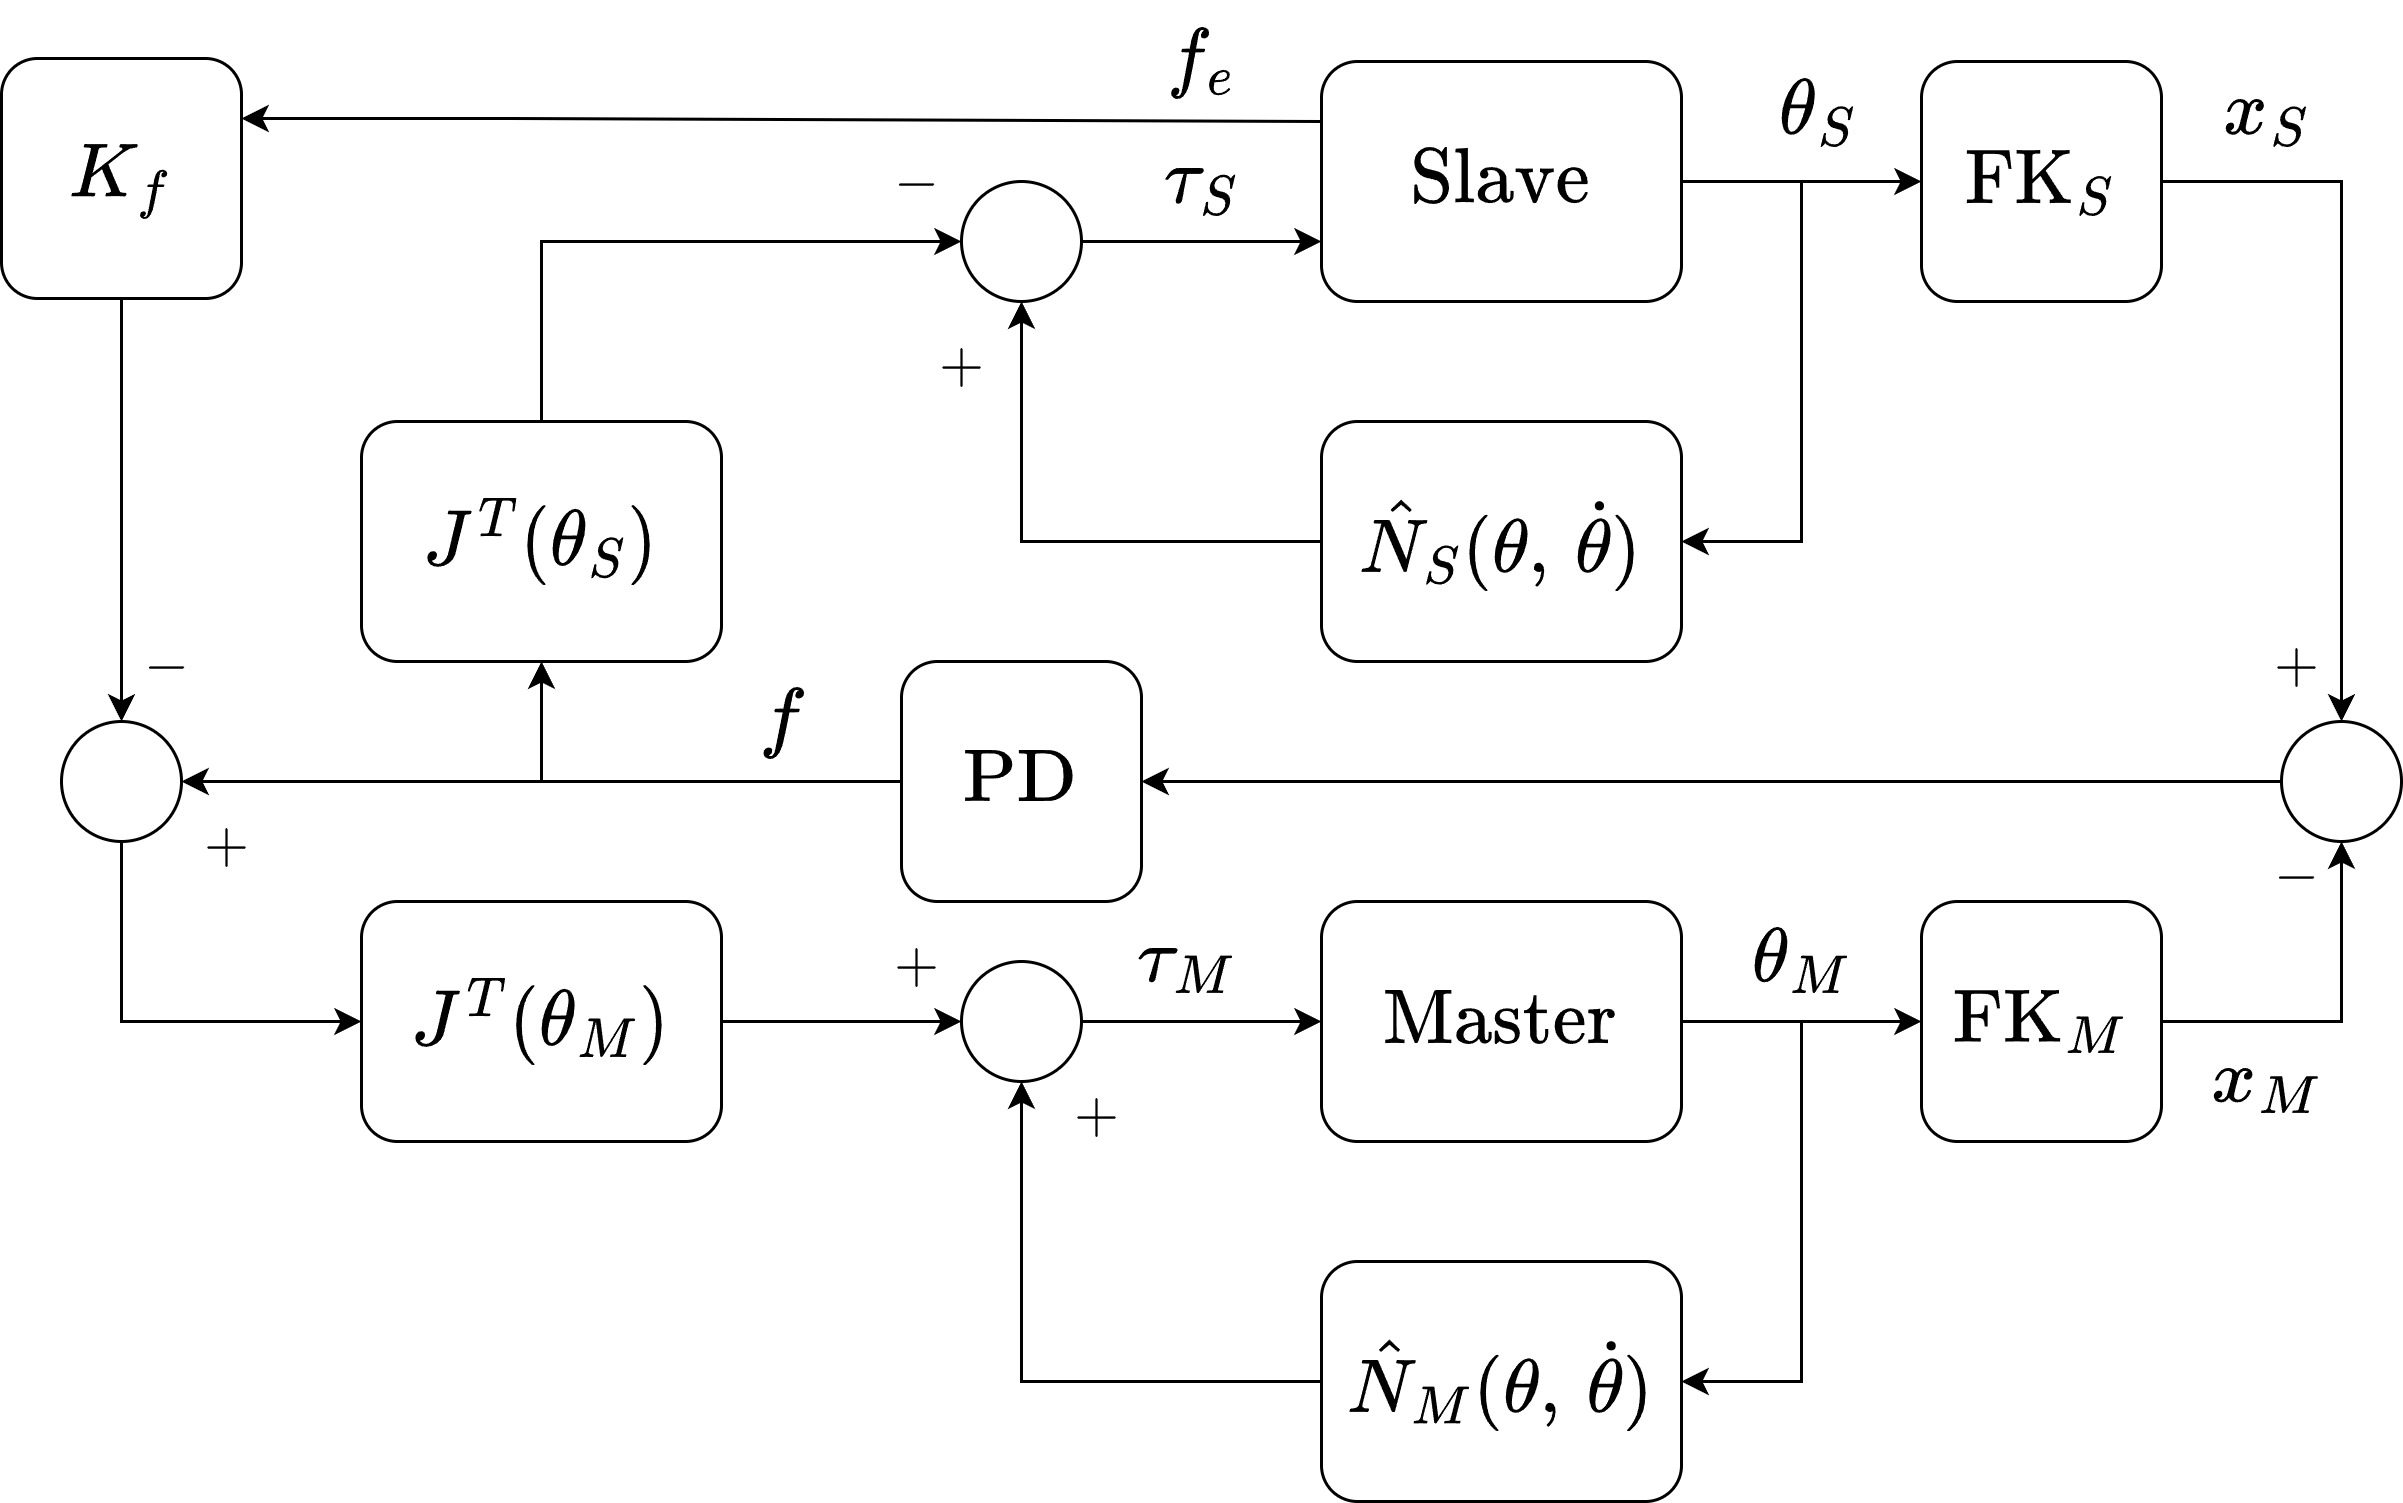
\includegraphics[width=\textwidth]{figures/bilateral_servo_direct_force_op_space.jpg}
    \end{subfigure}
\end{figure}





%%%%%%%
\begin{comment}
%%%%
\noindent\underline{}
\begin{figure}[h!]
    \centering
    \includegraphics[height=1.5in]{figures/}
\end{figure}
\end{comment}
%%%%%%%


\noindent\underline{Types of Force Control}
\begin{table}[h!]
    \footnotesize
    \centering
    \begin{tabular}{l|l|l}
         & Force Feedback & No Force Feedback  \\
         \hline
         Direct & Direct Force Control & FF Force Control\\
         \hline
         Indirect & Impedance/Admittance & Stiffness Control
    \end{tabular}
\end{table}

%%%
\noindent\underline{Relative Task Space}\\
Jacobians map wrenches \(\prescript{a}{}{w} = \prescript{a}{}{J}^T_b \prescript{b}{}{w}\)
\begin{equation*}
    \begin{bmatrix}
        \dot{x}_1 \\ \dot{x}_{\text{rel}}
    \end{bmatrix} = \begin{bmatrix}
        J_1 & 0 \\ -J_1 & J_2
    \end{bmatrix}\begin{bmatrix}
        \dot{\theta}_1 \\\dot{\theta}_2 
    \end{bmatrix} = J_{\text{rel}} \begin{bmatrix}
        \dot{\theta}_1 \\\dot{\theta}_2 
    \end{bmatrix}  \hspace{30pt} \begin{bmatrix}
        \tau_1 \\\tau_2
    \end{bmatrix} = J^T_{\text{rel}} \begin{bmatrix}
        f_{\text{ext}} \\ f_{\text{int}}
    \end{bmatrix}
\end{equation*}


%%%
\noindent\underline{Constraint Table}\\
All components of task-space must show up in each col, and row. 
\begin{table}[h!]
    \footnotesize
    \centering
    \begin{tabular}{l|l|l}
         & Kinematic & Static \\
         \hline
        Natural & keep obj. together & frictionless env. \\
        \hline
        Artificial & pos. control & force control 
    \end{tabular}
\end{table}


\end{document}